% \documentclass[12pt, a4paper, oneside]{ctexart}
\documentclass[12pt, oneside]{ctexart}
\usepackage{amsmath, amsthm, amssymb, bm, color, enumerate, framed, graphicx, longtable, mathrsfs, subfigure, tikz, ulem}
% \usepackage[dvipsnames]{xcolor}
% \usepackage{geometry}
\usepackage[a4paper, total={145mm,210mm}]{geometry}
\geometry{left=2.54cm,right=2.54cm,top=3.18cm,bottom=3.18cm}
\usepackage{pdfpages}

%按章节编号
\numberwithin{figure}{section}
\numberwithin{table}{section}

% 超链接设置
\usepackage{hyperref}
\hypersetup{  
    colorlinks = true,     % 更改链接颜色  
    linkcolor = purple,    % 链接颜色  
    urlcolor = blue,       % URL 颜色  
    citecolor = darkgreen, % 引用颜色  
    % underline = true,  
    linkbordercolor = red,
}
% \hypersetup{colorlinks=true,linkcolor=black}

% 自定义代码格式,与listings无关
\usepackage{fancyvrb}

%代码包设置
\usepackage{listings}
\lstset{
    basicstyle          =   \sffamily,          % 基本代码风格
    keywordstyle        =   \bfseries,          % 关键字风格
    commentstyle        =   \rmfamily\itshape,  % 注释的风格,斜体
    stringstyle         =   \ttfamily,  % 字符串风格
    flexiblecolumns,                % 别问为什么,加上这个
    numbers             =   left,   % 行号的位置在左边
    showspaces          =   false,  % 是否显示空格,显示了有点乱,所以不现实了
    numberstyle         =   \zihao{-5}\ttfamily,    % 行号的样式,小五号,tt等宽字体
    showstringspaces    =   false,
    captionpos          =   t,      % 这段代码的名字所呈现的位置,t指的是top上面
    frame               =   lrtb,   % 显示边框
}
% \lstdefinestyle{C}{
%     language        =   C, % 语言选C
%     basicstyle      =   \zihao{-5}\ttfamily,
%     numberstyle     =   \zihao{-5}\ttfamily,
%     keywordstyle    =   \color{blue},
%     keywordstyle    =   [2] \color{teal},
%     stringstyle     =   \color{magenta},
%     commentstyle    =   \color{red}\ttfamily,
%     breaklines      =   true,   % 自动换行,建议不要写太长的行
%     columns         =   fixed,  % 如果不加这一句,字间距就不固定,很丑,必须加
%     basewidth       =   0.5em,
% }
\lstdefinestyle{SQL}{
    language        =   SQL, % 语言选C
    basicstyle      =   \zihao{-5}\ttfamily,
    numberstyle     =   \zihao{-5}\ttfamily,
    keywordstyle    =   \color{blue},
    keywordstyle    =   [2] \color{teal},
    stringstyle     =   \color{magenta},
    commentstyle    =   \color{red}\ttfamily,
    breaklines      =   true,   % 自动换行,建议不要写太长的行
    columns         =   fixed,  % 如果不加这一句,字间距就不固定,很丑,必须加
    basewidth       =   0.5em,
}


% 设置思源宋体为中文字体
\setCJKsansfont{Source Han Serif SC}

% 设置思源黑体为中文字体
\setCJKsansfont{Source Han Sans SC}

% 设置arev为英文字体
\setsansfont{Arev Sans}

% 字体颜色
\def\red{\color{red}}
\def\blue{\color{blue}}
\def\black{\color{black}}
\def\green{\color{green}}

\CTEXsetup[format={\Large\bfseries}]{section}

\definecolor{shadecolor}{RGB}{241, 241, 255}
\newcounter{problemname}
\newenvironment{problem}{\begin{shaded}\stepcounter{problemname}\par\noindent\textbf{题目\arabic{problemname}. }}{\end{shaded}\par}
\newenvironment{solution}{\par\noindent\textbf{解答. }}{\par}
\newenvironment{note}{\par\noindent\textbf{题目\arabic{problemname}的注记. }}{\par}
%\renewcommand{\proofname}{\bf 证明}

\begin{document}

\thispagestyle{empty}

\begin{figure}[t]
    \centering
    
\includegraphics[width=13cm]{images/logo.png}
\end{figure}

\vspace*{\fill}
    \begin{center}
        \Huge\textbf{数据库原理}
    \end{center}
    \rightline{\LARGE\textbf{——课程作业}}
\vspace*{\fill}

\begin{table}[b]
    \centering
    \large
    \begin{tabular}{ll}
    \textbf{课程:} & 数据库原理 \\
    \textbf{班级:} & 1621402 \\
    \textbf{姓名:} & 黄钰轩 \\
    \textbf{学号:} & 162140222 \\
    \textbf{教师:} & 郑吉平 \\
    \textbf{学期:} & 2023-2024 春季 \\
    \end{tabular}
\end{table}

\newpage
\pagenumbering{Roman}
\setcounter{page}{1}
\tableofcontents
\newpage
\setcounter{page}{1}
\pagenumbering{arabic}

\section{第一章作业}

\begin{problem}
    试述数据、数据库、数据库管理系统、数据库系统的概念.
\end{problem}

\begin{solution}
    \begin{enumerate}[(1)]
        \item 数据: 描述事物的符号记录.
        \begin{itemize}
            \item 在现实生活,数据是可识别的抽象符号,即描述事物的符号记录.
            \item 在计算机中,数据是所有能被计算机处理的符号的总称.
            \item 在数据库中,数据是数据库中存储的基本对象.
        \end{itemize}
        \item 数据库: 
        \begin{itemize}
            \item 一组相互有关联的数据集合.
            \item 长期储存在计算机中的有组织的、可管理和可共享的数据集合.
        \end{itemize}
        \item 数据库管理系统:
        \begin{itemize}
            \item 位于用户(应用程序)与操作系统之间的数据库管理软件.
            \item 一个管理数据的大型复杂基础软件系统.
        \end{itemize}
        \item 数据库系统: 
        \begin{itemize}
            \item 由数据库管理系统和相关工具组成的软件系统,用于管理和操作大量数据.
        \end{itemize}
    \end{enumerate}
\end{solution}

\begin{problem}
    试述数据模型的概念、作用及其包含的三个要素.
\end{problem}

\begin{solution}
    \begin{enumerate}[(1)]
        \item 数据库模型的概念:
        \begin{itemize}
            \item 数据模型是数据库结构的基础,它是描述数据(数据结构)、数据之间的联系,数据语义即数据操作,以及一致性(完整性)约束的\textbf{概念和工具的集合}.
        \end{itemize}
        \item 数据库模型的作用:
        \begin{itemize}
            \item 在数据库领域,数据模型被广泛用于表示这些数据库设计的“描述”,更好的刻画数据.
            \item 数据模型精确描述了系统的静态特性、动态特性和完整性约束条件.
        \end{itemize}
        \item 数据库模型的三个要素:
        \begin{itemize}
            \item 数据结构: 数据结构描述数据库的组成对象以及对象之间的联系.
            \item 数据操纵: 是指对数据库中各种对象(型)的实例(值)允许进行的操作的集合,包括操作及有关的操作规则,是对系统动态特性的描述.
            \item 完整性约束: 是一组完整性规则的集合. 完整性规则是给定的数据模型中数据及其联系所具有的制约和依存规则,用以限定符合数据模型的数据库状态以及状态的变化,以保证数据的正确、有效、相容.
        \end{itemize}
    \end{enumerate}
\end{solution}

\begin{problem}
    试述数据库系统的三级模式结构,并说明这种结构的优点是什么.
\end{problem}

\begin{solution}
    \begin{enumerate}[(1)]
        \item 数据库系统的三级模式结构由模式、外模式和内模式组成.
        \begin{itemize}
            \item 模式也称逻辑模式,是数据库中全体数据的逻辑结构和特征的描述,是所有用户的公共数据视图. 模式的一个具体值称为模式的一个实例.
            \item 外模式,亦称子模式或用户模式,是数据库用户(包括应用程序员和最终用户)能够看见和使用的局部数据的逻辑结构和特征的描述,是数据库用户的数据视图,是与某一应用有关的数据的逻辑表示.
            \item 内模式也称物理模式或存储模式,它是对数据物理结构和存方式的描述,是数据在数据库内部的组织方式.
        \end{itemize}
        \item 三级模式结构的优点:
        \begin{itemize}
            \item 数据库系统的三级模式是对数据的三个抽象级别,它把数据的具体组织留给数据库管理系统,使用户能逻辑抽象地处理数据,而不必关心数据在计算机中的具体表示方式和存储方式.
            \item 数据库系统在这三级模式之间提供了两层映像: 外模式/模式映像和模式/内模式映像. 正是这两层映像保证了数据库系统中的数据能够具有较高的逻辑独立性和物理独立性.
        \end{itemize}
    \end{enumerate}
\end{solution}

\begin{problem}
    试述数据与程序的物理独立性和逻辑独立性. 为什么数据库系统具有较强的数据与程序的独立性?
\end{problem}

\begin{solution}
    \begin{enumerate}[(1)]
        \item 
        \begin{itemize}
            \item 数据与程序的物理独立性: 当数据库的存储结构改变时(如选用了另一种存储结构),由数据库管理员对模式/内模式映像做相应改变,可以使模式保持不变,从而应用程序也不必改变,保证了数据与程序的物理独立性,简称数据的物理独立性.
            \item 数据与程序的逻辑独立性: 当模式改变时(例如增加新的关系、新的属性、改变属性的数据类型等),由数据库管理员对各个外模式/模式的映像做相应改变,可以使外模式保持不变. 应用程序是依据数据的外模式编写的,从而应用程序不必修改,保证了数据与程序的逻辑独立性,简称数据的逻辑独立性.
        \end{itemize}
        \item 数据库管理系统在三级模式之间提供的两层映像保证了数据库系统中的数据能够具有较高的逻辑独立性和物理独立性.
    \end{enumerate}
\end{solution}

\newpage
\section{第二章作业}
% 计数器置零
\setcounter{problemname}{0}

\begin{problem}
    试述关系模型的三个组成部分.
\end{problem}

\begin{solution}
    关系模型由关系数据结构、关系操作集合和关系完整性约束三部分组成.
    \begin{figure}[!htpb]
        \centering
        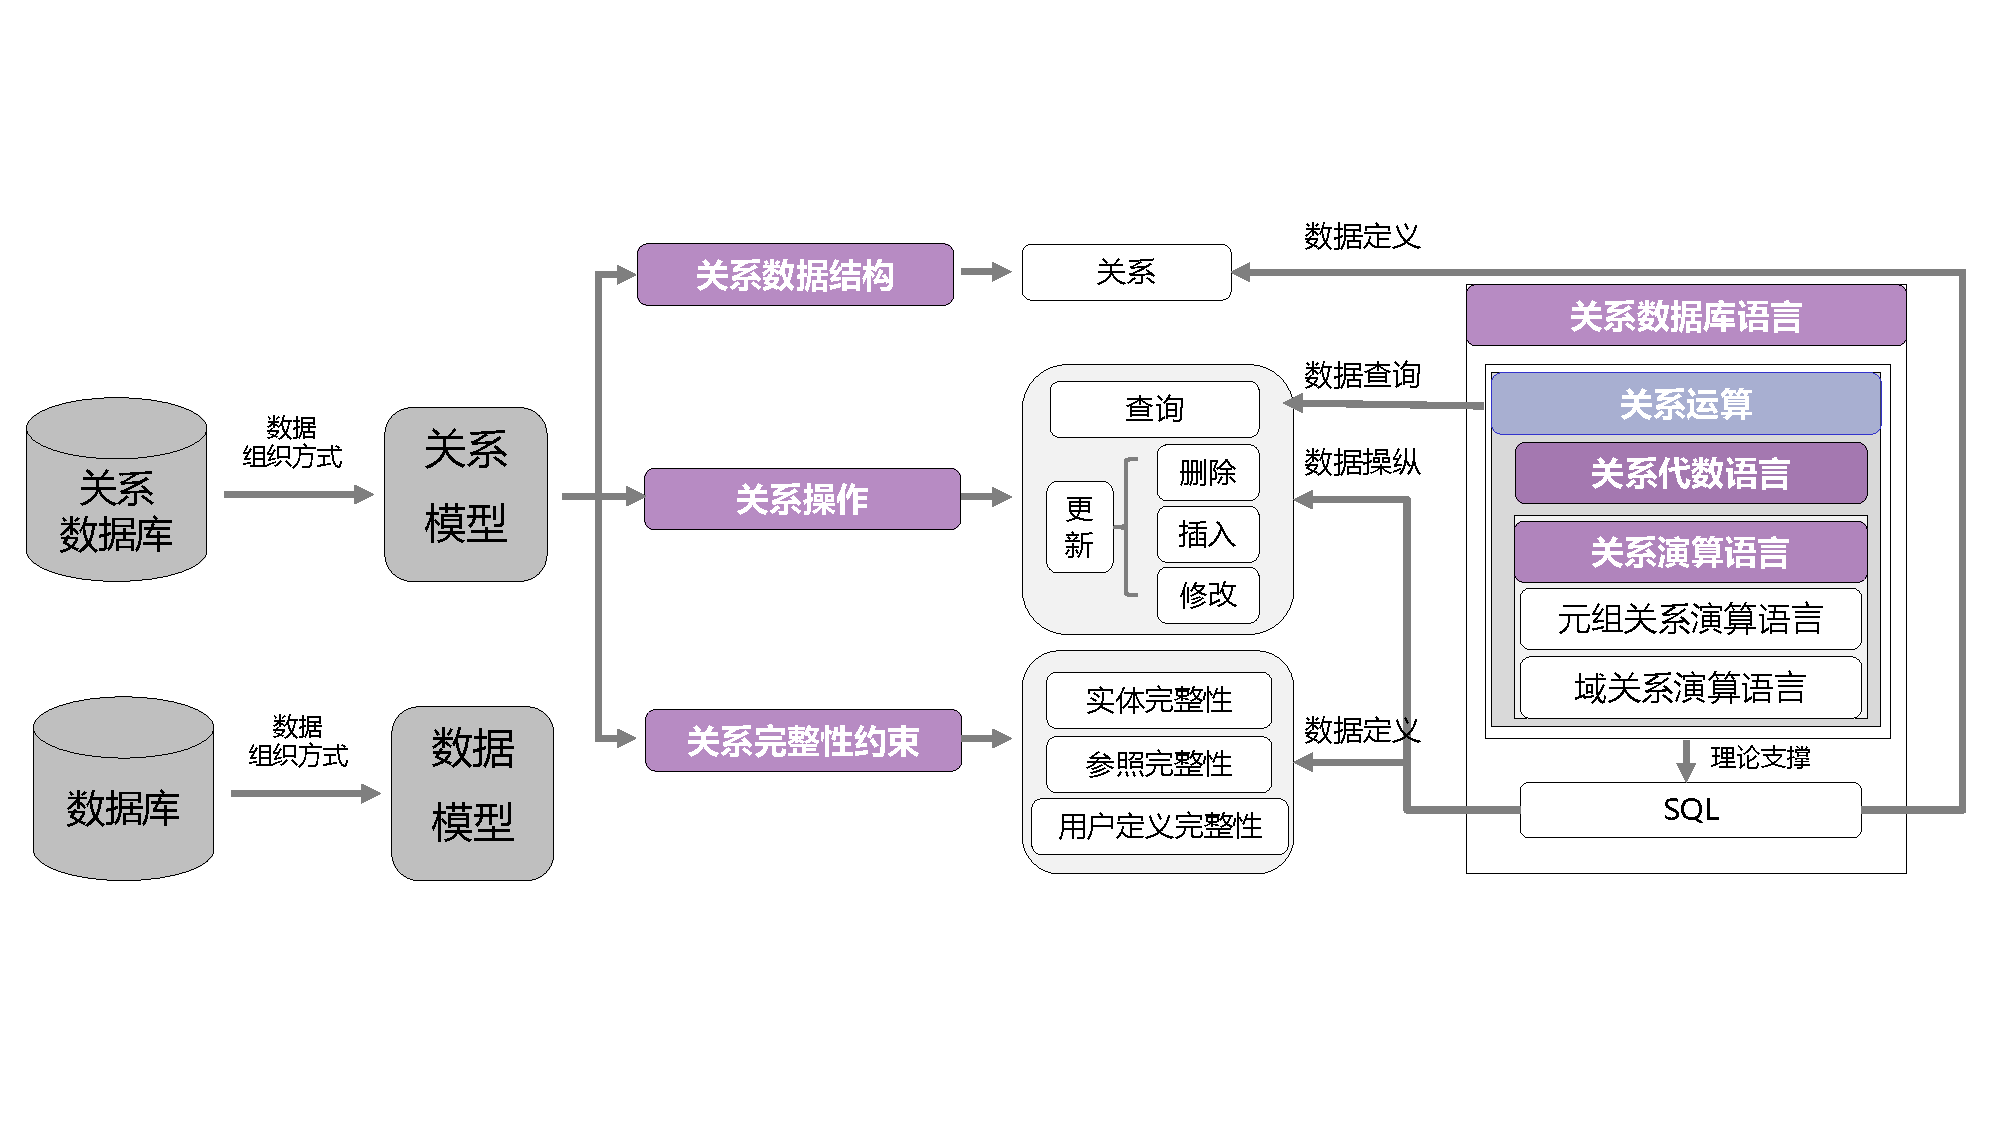
\includegraphics[width=15.5cm]{images/sec2/2-1_Relational_Model.pdf}
        \caption{关系模型框架}
        \label{fig2-1}
    \end{figure}
\end{solution}

\begin{problem} \label{2-6}
    设有一个$\mathbf{SPJ}$数据库,包括四个关系模式 $\mathbf{S}$、$\mathbf{P}$、$\mathbf{J}$ 和$\mathbf{SPJ}$.
    $$\begin{aligned}
        & \mathrm{S(SNO, SNAME, STATUS, CITY);}  \\
        & \mathrm{P(PNO, PNAME, COLOR, WEIGHT);} \\
        & \mathrm{J(JNO, JNAME, CITY);}          \\
        & \mathrm{SPJ(SNO, PNO, JNO, QTY)}.
    \end{aligned}$$

    供应商表$\mathbf{S}$由供应商代码(SNO)、供应商姓名(SNAME)、供应商状态(STATUS)、供应商所在城市(CITY)组成.

    零件表$\mathbf{P}$由零件代码(PNO)、零件名(PNAME)、颜色(COLOR)、重量(WEIGHT)组成.

    工程项目表$\mathbf{J}$由工程项目代码(JNO)、工程项目名(JNAME)、工程项目所在城市(CITY)组成.

    供应情况表$\mathbf{SPJ}$由供应商代码(SNO)、零件代码(PNO)、工程项目代码(JNO)、供应数量(QTY)组成,表示某供应商供应某种零件给某工程项目的数量为QTY.

    今有若干数据如 图 \ref{SPJ} 所示.

    试用关系代数、元组关系演算语言 ALPHA 完成如下查询:
    \begin{enumerate}[(1)]
        \item 求供应工程 J1 零件的供应商代码 SNO.
        \item 求供应工程 J1 零件 P1 的供应商代码 SNO.
        \item 求供应工程 J1 零件为红色的供应商代码 SNO.
        \item 求没有使用天津供应商生产的红色零件的工程号 JNO.
        \item 求至少使用了与供应商 S1 所供应的全部零件相同零件号的工程号 JNO.
    \end{enumerate}
\end{problem}

\begin{figure}[!htpb]
    \centering
    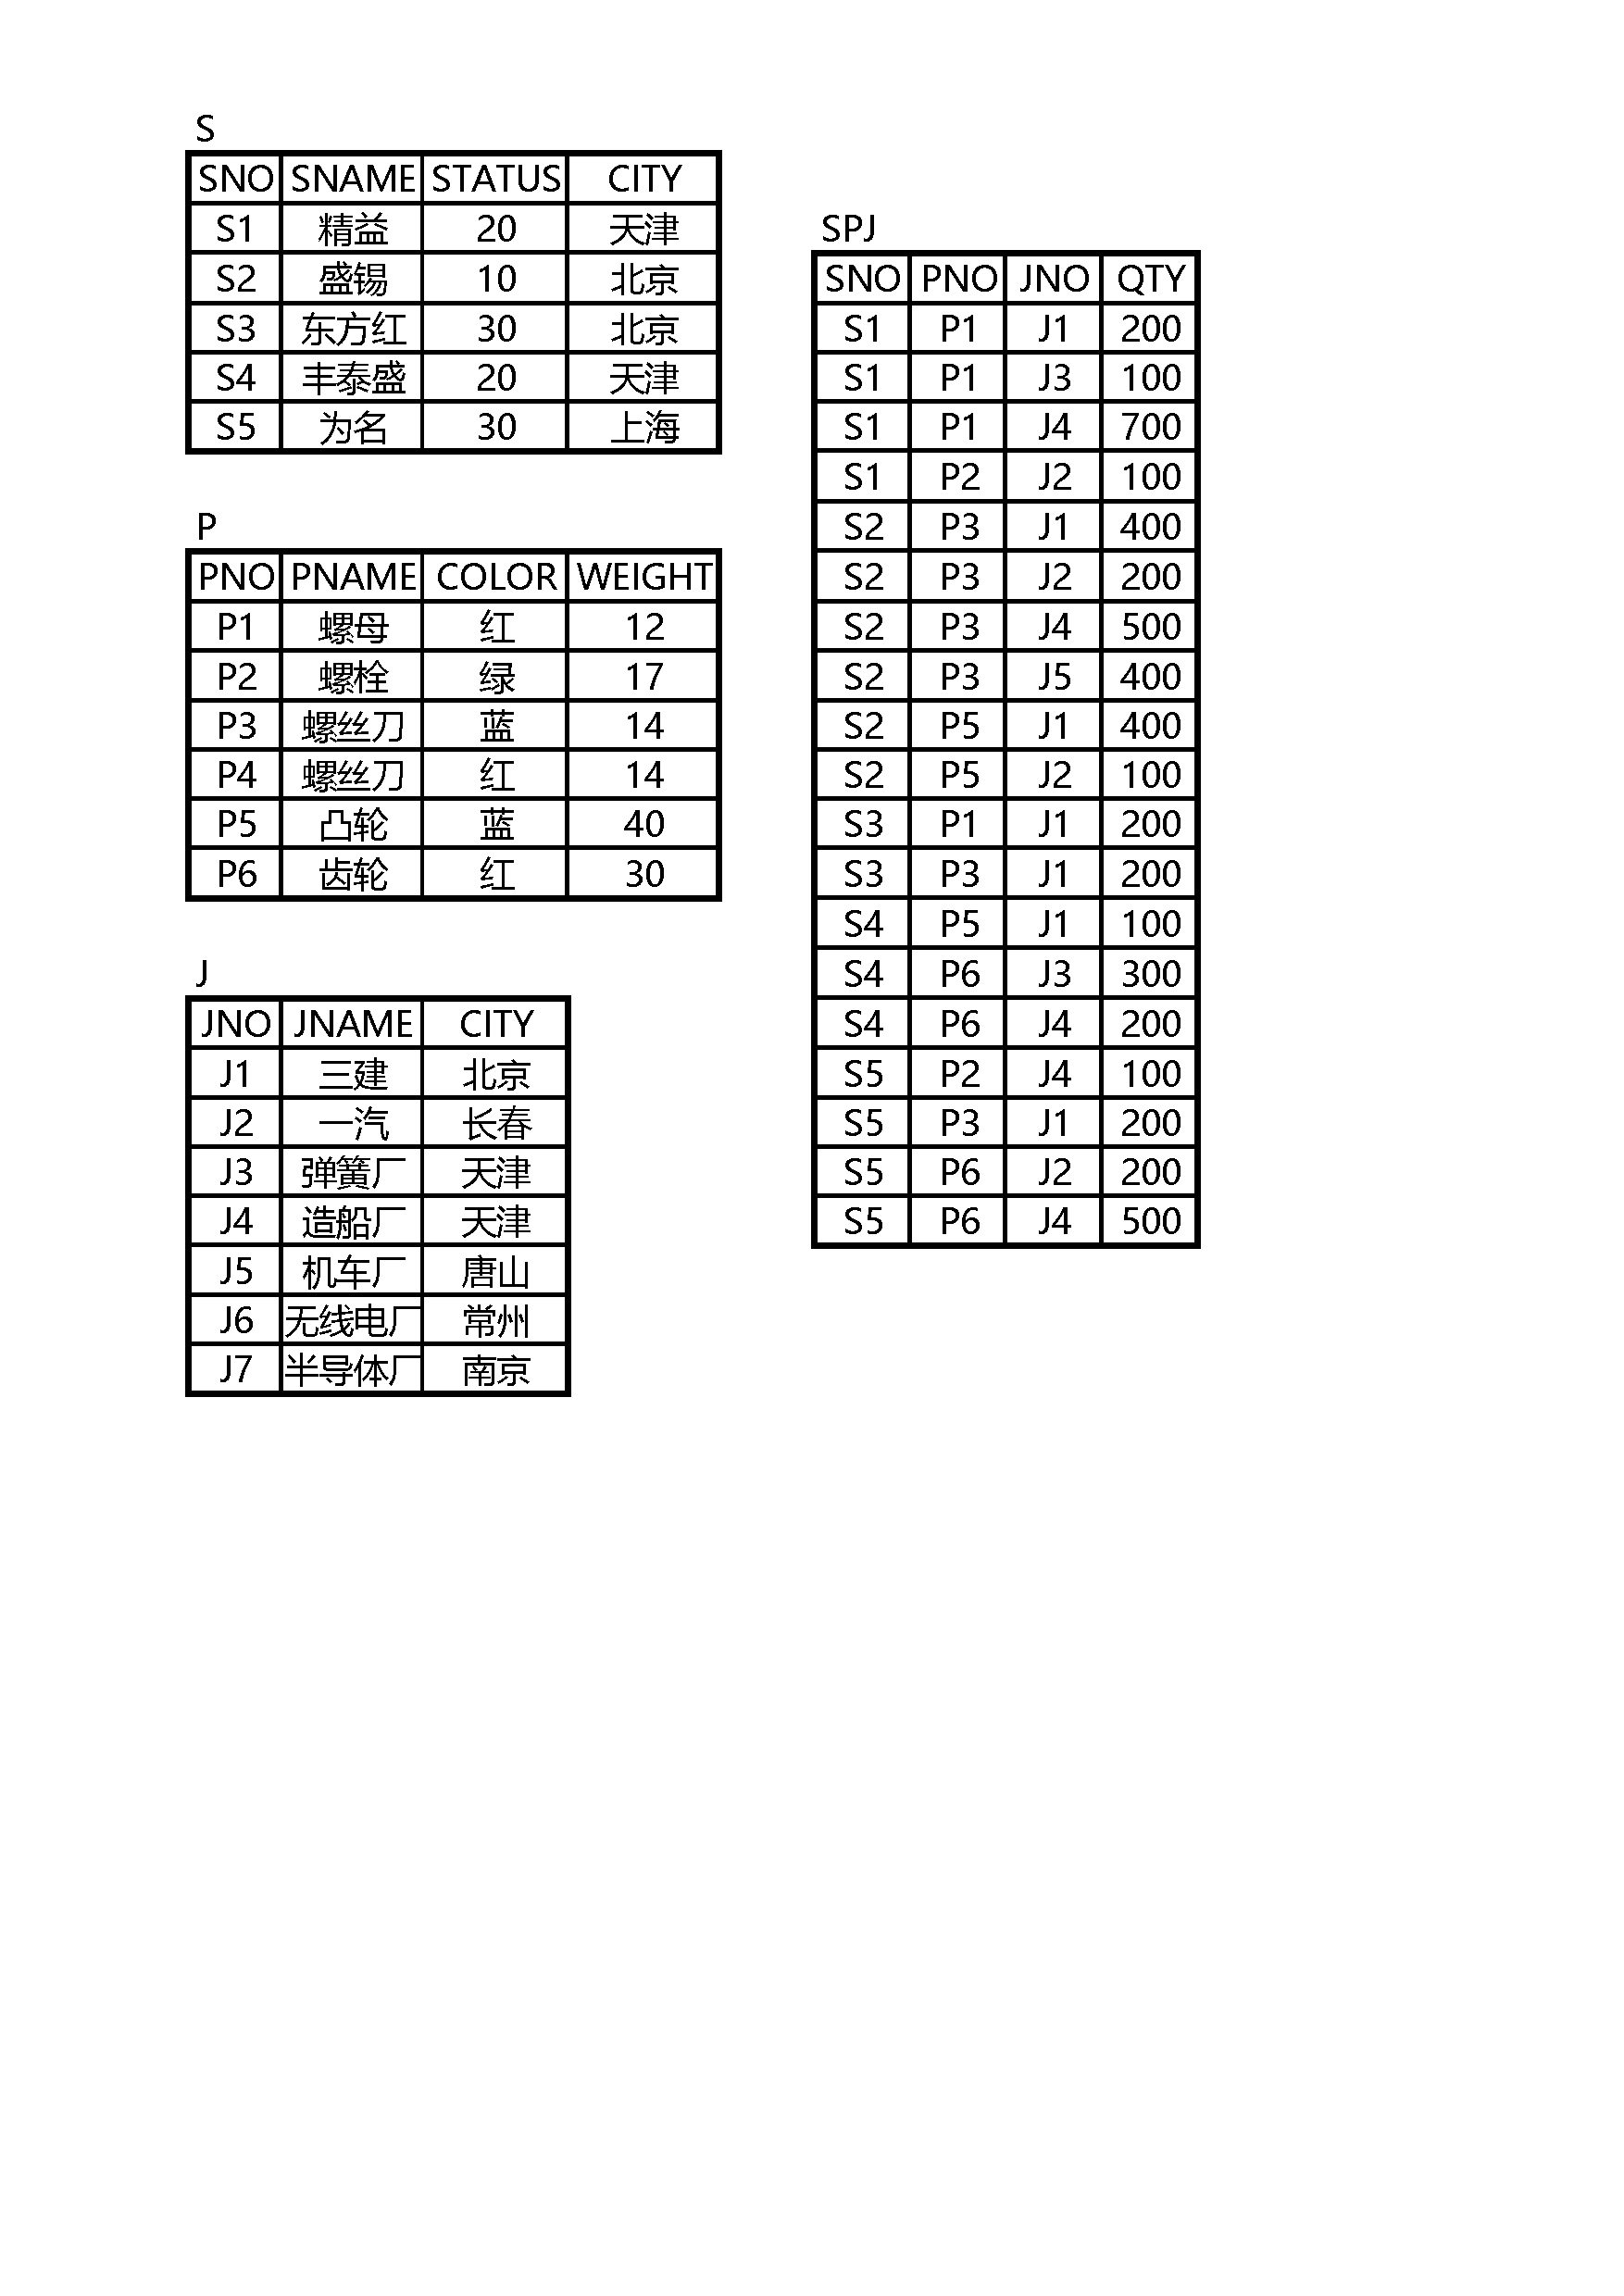
\includegraphics[width=13cm]{images/sec2/2-2_SPJ.pdf}
    \caption{SPJ 数据库数据}
    \label{SPJ}
\end{figure}

\begin{solution}
    \begin{enumerate}[(1)]
        \item
        \begin{itemize}
            \item 关系代数:
                  $$\Pi_{\mathrm{SNO}}(\sigma_{\mathrm{JNO} = '\mathrm{J1}'}(\mathbf{SPJ}))$$
            \item ALPHA语言:
                \lstinputlisting[
                    % style       =   C,
                    % caption     =   {\bf probe.c},
                    label       =   {3-1_code}
                ]{./code/sec2/3-1.txt}
        \end{itemize}
        \item
        \begin{itemize}
            \item 关系代数:
                  $$\Pi_{\mathrm{SNO}}(\sigma_{\mathrm{JNO} = '\mathrm{J1}' \land \mathrm{PNO} = '\mathrm{P1}'}(\mathbf{SPJ}))$$
            \item ALPHA语言:
                \lstinputlisting[
                    % style       =   C,
                    % caption     =   {\bf probe.c},
                    label       =   {3-2_code}
                ]{./code/sec2/3-2.txt}
        \end{itemize}
        \item
        \begin{itemize}
            \item 关系代数:
                  $$\Pi_{\mathrm{SNO}}(\Pi_{\mathrm{SNO}, \mathrm{PNO}}(\sigma_{\mathrm{JNO} = '\mathrm{J1}'}(\mathbf{SPJ})) \bowtie \Pi_{\mathrm{PNO}}(\sigma_{\mathrm{COLOR} = '\text{红}'}(\mathbf{P})))$$
            \item ALPHA语言:
                \lstinputlisting[
                        % style       =   C,
                        % caption     =   {\bf probe.c},
                        label       =   {3-3_code}
                    ]{./code/sec2/3-3.txt}
        \end{itemize}
        \item
        \begin{itemize}
            \item 关系代数:
            $$\Pi_{\mathrm{JNO}}(\mathbf{SPJ}) - \Pi_{\mathrm{JNO}}(\sigma_{\mathrm{CITY} = '\text{天津}' \land \mathrm{COLOR} = '\text{红}'}(\mathbf{S} \bowtie \mathbf{SPJ} \bowtie \mathbf{P}))$$
            \item ALPHA语言:
                \lstinputlisting[
                    % style       =   C,
                    % caption     =   {\bf probe.c},
                    label       =   {3-4_code}
                ]{./code/sec2/3-4.txt}
            \end{itemize}
        \item
        \begin{itemize}
            \item 关系代数:
                  $$\Pi_{\text{JNO},\text{PNO}}(\mathbf{SPJ}) \div \Pi_{\text{PNO}}(\sigma_{\text{SNO} = '\text{S1}'}(\mathbf{SPJ}))$$
            \item ALPHA语言:
                \lstinputlisting[
                    % style       =   C,
                    % caption     =   {\bf probe.c},
                    label       =   {3-5_code}
                ]{./code/sec2/3-5.txt}
        \end{itemize}
    \end{enumerate}
\end{solution}

\begin{problem}
    试述等值连接与自然连接的区别和联系.
\end{problem}

\begin{solution}
    \begin{itemize}
        \item 自然连接是一种特殊的等值连接.
        \item 自然连接将连接条件指定为$R$和$S$中属性名相同的列做等值连接,因此$p$可省略.
    \end{itemize}
\end{solution}
\newpage
\begin{note}
    以$\mathbf{Student}$、$\mathbf{SC}$表为例,
    $$\mathbf{Student}\bowtie_{\mathrm{Student.Sno = SC.Sno}}\mathbf{SC}$$
    结果如下:
    \begin{figure}[!htpb]
        \centering
        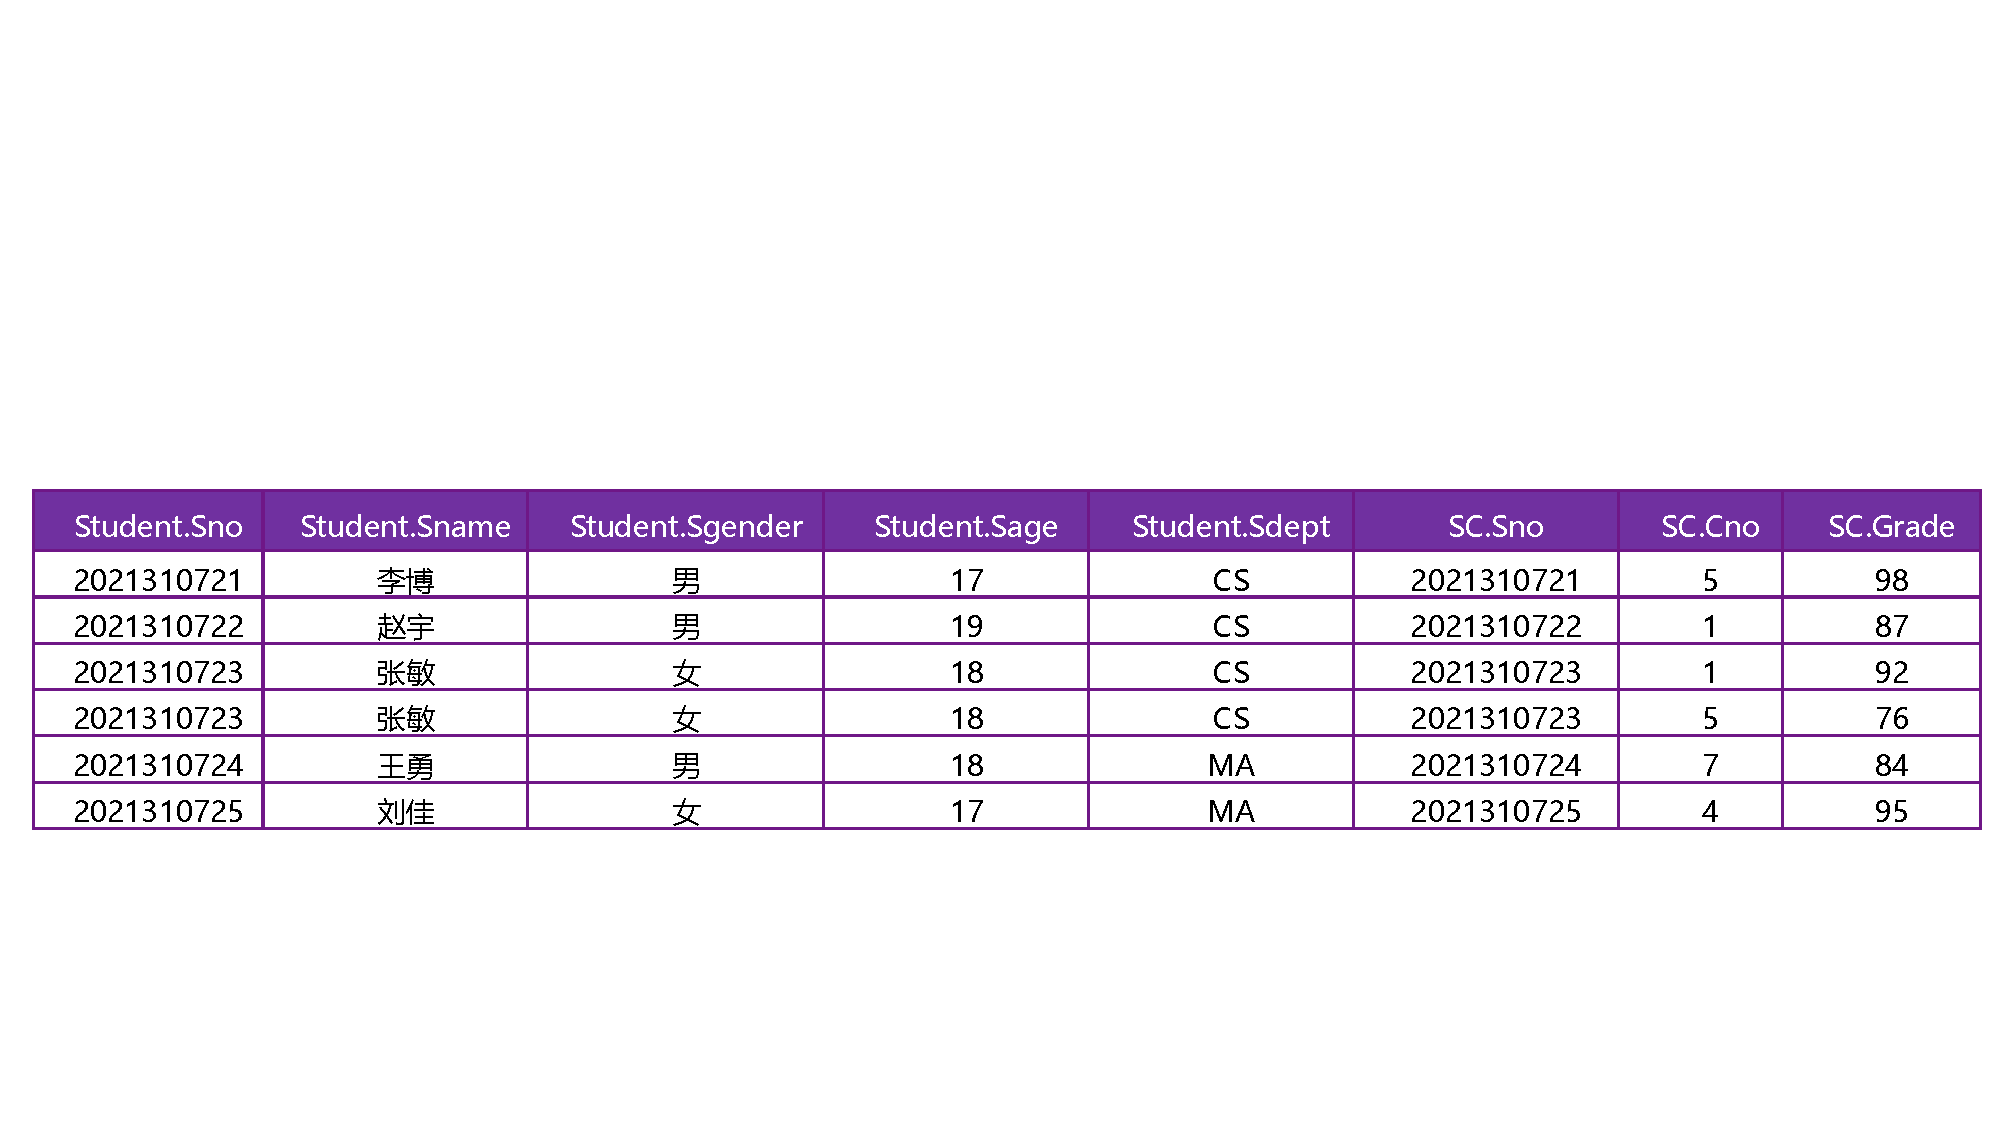
\includegraphics[width=15cm]{images/sec2/2-3_Equijoin.pdf}
        \caption{等值连接}
        \label{fig2-3_1}
    \end{figure}

    而
    $$\mathbf{Student}\bowtie\mathbf{SC}$$
    结果如下:
    \begin{figure}[!htpb]
        \centering
        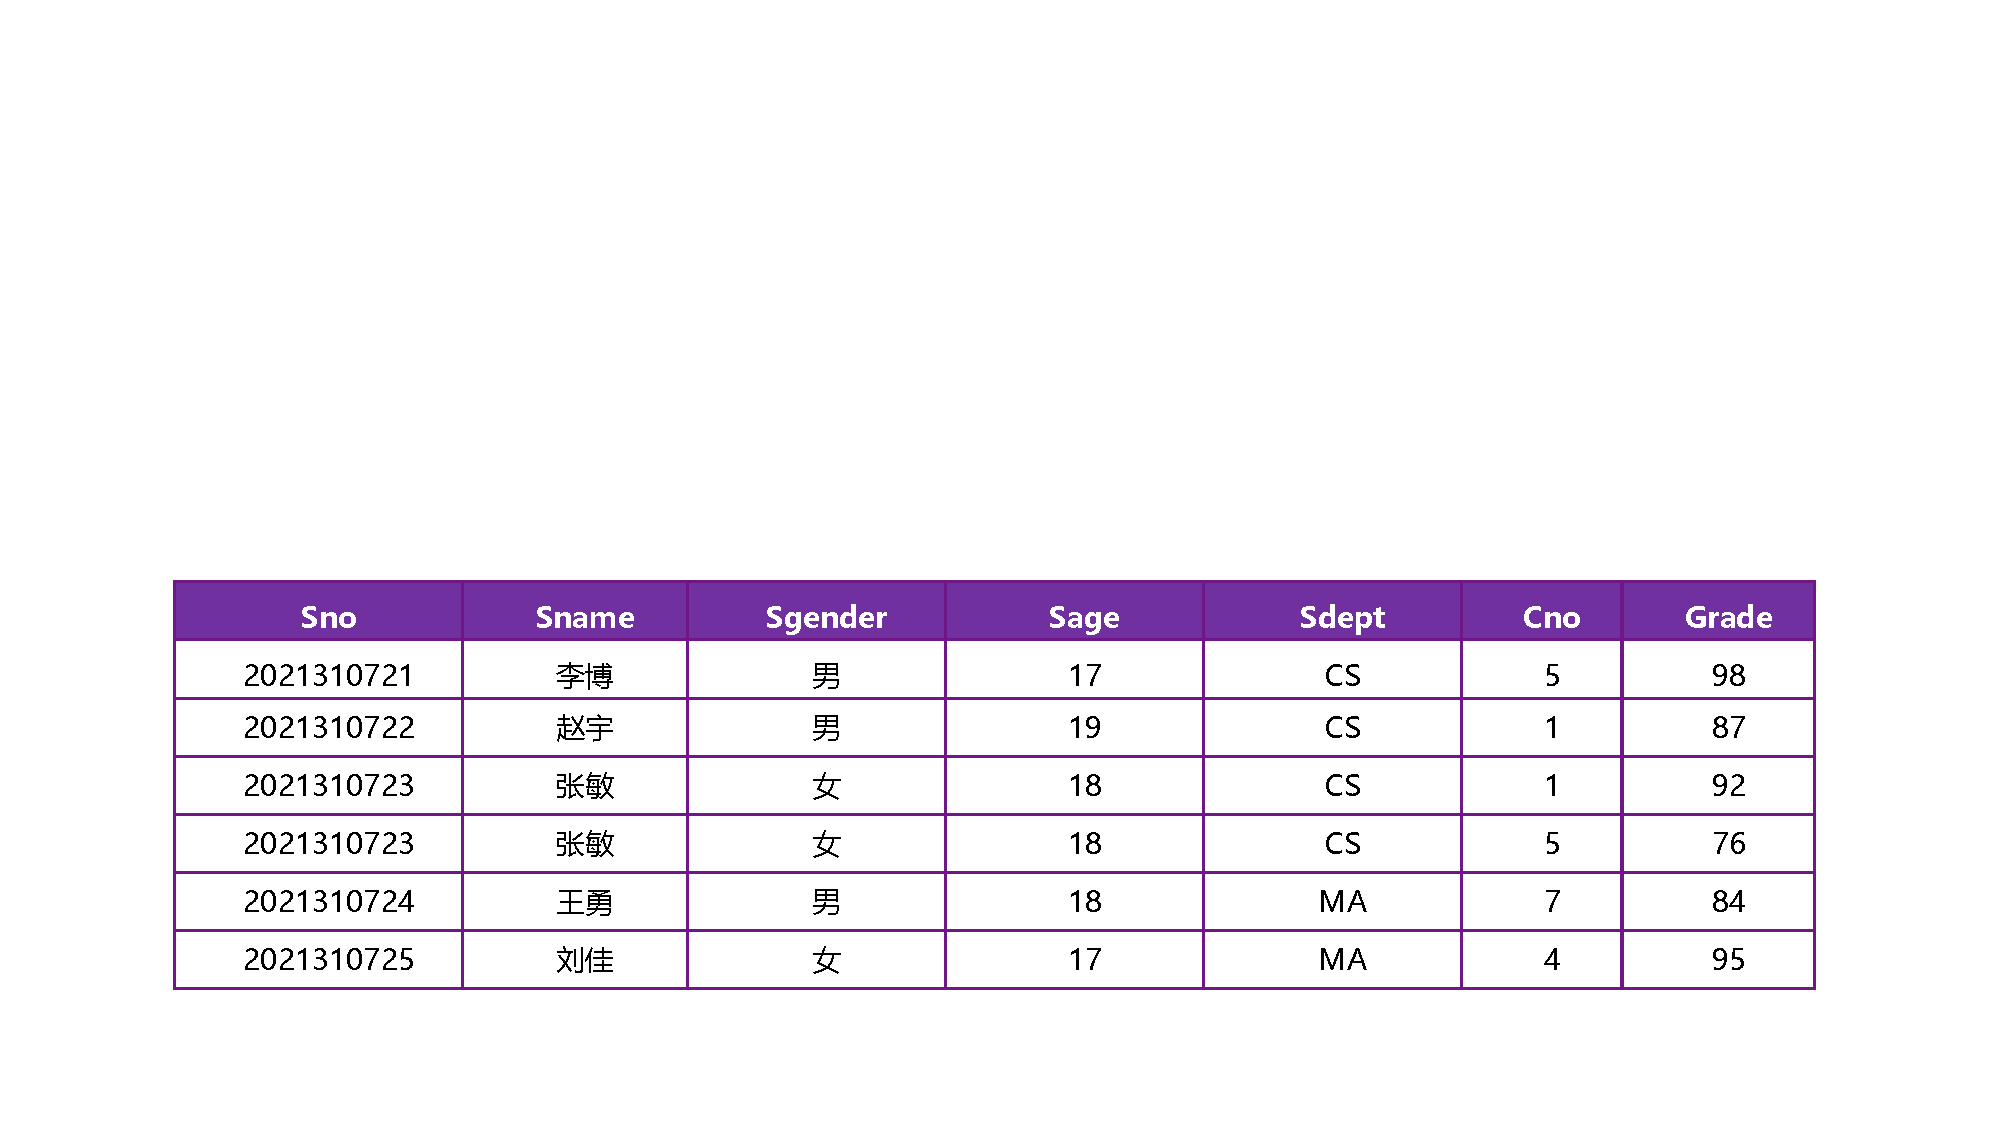
\includegraphics[width=15cm]{images/sec2/2-3_Natural_Join.pdf}
        \caption{自然连接}
        \label{fig2-3_2}
    \end{figure}
\end{note}

\begin{problem}
    关系代数的基本运算有哪些? 如何用这些基本运算来表示其他运算?
\end{problem}

\begin{solution}
    \begin{itemize}
        \item 基本运算:
        \begin{itemize}
            \item 选择($\sigma$):
                  $$\sigma_p(R) = \{t | t \in R \land p(t) = True\}$$
            \item 投影($\Pi$):
                  $$\Pi_{A_1,A_2,\ldots,A_k}(R) = \{t[A_1,A_2,\ldots,A_k] | t \in R\}$$
            \item 并($\bigcup$):
                  $$R\bigcup S = \{t | t\in R \lor t \in S\}$$
            \item 差($-$):
                  $$R - S = \{t | t\in R \land t \notin S\}$$
            \item 笛卡尔积($\times$):
                  $$R \times S = \{(t, q) | t\in R \land q \in S\}$$
        \end{itemize}
        \item 附加运算:
        \begin{itemize}
            \item 交($\bigcap$):
                  $$R\bigcap S = \{t | t\in R \land t \in S\}$$
                  满足:
                  $$R\bigcap S = R - (R - S)$$
            \item 连接($\bowtie$):
                  $$R\bowtie_p S = \{(t, q) | t \in R \land q \in S \land p\left((t, q)\right) = True\}$$
                  满足:
                  $$R\bowtie_p S = \sigma_p(R \times S)$$
            \item 除($\div$): \\
                  设$R(A_1,A_2,\ldots,A_m, B_1,B_2,\ldots,B_n)$和$S(B_1,B_2,\ldots,B_n, C_1,C_2,\ldots,C_k)$ 是两个关系,则$R \div S$的属性为$A_1,A_2,\ldots,A_m$,且:
                  $$R \div S = \{t | t\in \Pi_{A_1,A_2,\ldots,A_m}(R) \land (\forall q \in \Pi_{B_1,B_2,\ldots,B_n}(S), (t, q) \in R)\}$$
                  满足:
                  $$R \div S = \Pi_{A_1,A_2,\ldots,A_m}(R) - \Pi_{A_1,A_2,\ldots,A_m}((\Pi_{A_1,A_2,\ldots,A_m}(R) \times \Pi_{B_1,B_2,\ldots,B_n}(S)) - R)$$
        \end{itemize}
    \end{itemize}
\end{solution}

\newpage
\section{第三章作业}
% 计数器置零
\setcounter{problemname}{0}

\begin{problem}
    有两个关系 $\mathbf{S}(A, B, C, D)$ 和 $\mathbf{T}(C, D, E, F)$, 写出与下列查询等价的 SQL 表达式:
    \begin{enumerate}[(1)]
        \item $\sigma_{A = 10}(\mathbf{S})$.
        \item $\Pi_{A, B}(\mathbf{S})$.
        \item $\mathbf{S} \bowtie \mathbf{T}$.
        \item $\mathbf{S} \mathop{\bowtie}\limits_{\mathbf{S}.C = \mathbf{T}.C} \mathbf{T}$.
        \item $\mathbf{S} \mathop{\bowtie}\limits_{A < E} \mathbf{T}$.
        \item  $\Pi_{C, D}(\mathbf{S}) \times \mathbf{T}$.
    \end{enumerate}
\end{problem}

\begin{solution}
    \begin{enumerate}[(1)]
        \item \ 
            \lstinputlisting[
                style       =   SQL,
                % caption     =   {\bf probe.c},
                label       =   {3-1-1_code}
            ]{./code/sec3/3-1-1.sql}
        \item \ 
            \lstinputlisting[
                style       =   SQL,
                % caption     =   {\bf probe.c},
                label       =   {3-1-2_code}
            ]{./code/sec3/3-1-2.sql}
        \item \ 
            \lstinputlisting[
                style       =   SQL,
                % caption     =   {\bf probe.c},
                label       =   {3-1-3_code}
            ]{./code/sec3/3-1-3.sql}
        \item \ 
            \lstinputlisting[
                style       =   SQL,
                % caption     =   {\bf probe.c},
                label       =   {3-1-4_code}
            ]{./code/sec3/3-1-4.sql}
        \item \ 
            \lstinputlisting[
                style       =   SQL,
                % caption     =   {\bf probe.c},
                label       =   {3-1-5_code}
            ]{./code/sec3/3-1-5.sql}
        \item \ 
            \lstinputlisting[
                style       =   SQL,
                % caption     =   {\bf probe.c},
                label       =   {3-1-6_code}
            ]{./code/sec3/3-1-6.sql}
    \end{enumerate}
\end{solution}

\begin{problem}
    使用 SQL 语句建立(\hyperref[2-6]{题目2-6})中 SPJ 数据库的四个表($\mathbf{S}$、$\mathbf{P}$、$\mathbf{J}$和$\mathbf{SPJ}$),并针对建立的四个表用 SQL 语句完成(\hyperref[2-6]{题目2-6})中的查询.
\end{problem}

\begin{solution}
    \begin{itemize}
        \item 建表:
            \begin{itemize}
                \item 建 $\mathbf{S}$ 表:
                    \lstinputlisting[
                        style       =   SQL,
                        % caption     =   {\bf probe.c},
                        label       =   {3-2-1_code}
                    ]{./code/sec3/3-2-1.sql}
                \item 建 $\mathbf{P}$ 表:
                    \lstinputlisting[
                        style       =   SQL,
                        % caption     =   {\bf probe.c},
                        label       =   {3-2-2_code}
                    ]{./code/sec3/3-2-2.sql}
                \item 建 $\mathbf{J}$ 表:
                    \lstinputlisting[
                        style       =   SQL,
                        % caption     =   {\bf probe.c},
                        label       =   {3-2-3_code}
                    ]{./code/sec3/3-2-3.sql}
                \newpage
                \item 建 $\mathbf{SPJ}$ 表:
                    \lstinputlisting[
                        style       =   SQL,
                        % caption     =   {\bf probe.c},
                        label       =   {3-2-4_code}
                    ]{./code/sec3/3-2-4.sql}
            \end{itemize}
        \item 查询:
            \begin{enumerate}[(1)]
                \item \ 
                    \lstinputlisting[
                        style       =   SQL,
                        % caption     =   {\bf probe.c},
                        label       =   {3-2-5_code}
                    ]{./code/sec3/3-2-5.sql}
                \item \ 
                    \lstinputlisting[
                        style       =   SQL,
                        % caption     =   {\bf probe.c},
                        label       =   {3-2-6_code}
                    ]{./code/sec3/3-2-6.sql}
                \item \ 
                    \lstinputlisting[
                        style       =   SQL,
                        % caption     =   {\bf probe.c},
                        label       =   {3-2-7_code}
                    ]{./code/sec3/3-2-7.sql}
                \item \ 
                    \lstinputlisting[
                        style       =   SQL,
                        % caption     =   {\bf probe.c},
                        label       =   {3-2-8_code}
                    ]{./code/sec3/3-2-8.sql}
                \newpage
                \item \ 
                    \lstinputlisting[
                        style       =   SQL,
                        % caption     =   {\bf probe.c},
                        label       =   {3-2-9_code}
                    ]{./code/sec3/3-2-9.sql}
            \end{enumerate}
    \end{itemize}
\end{solution}

\begin{problem}
    针对(\hyperref[2-6]{题目2-6})中的四个表($\mathbf{S}$、$\mathbf{P}$、$\mathbf{J}$和$\mathbf{SPJ}$),试用 SQL 完成以下各项操作:
    \begin{enumerate}[(1)]
        \item 找出所有供应商的姓名和所在城市.
        \item 找出所有零件的名称、颜色、重量.
        \item 找出使用供应商 S1 所供应零件的工程代码.
        \item 找出工程项目 J2 使用的各种零件的名称及其数量.
        \item 找出上海厂商供应的所有零件代码.
        \item 找出使用上海产的零件的工程名称.
        \item 找出没有使用天津产的零件的工程代码.
        \item 把全部红色零件的颜色改成蓝色.
        \item 把由 S5 供给 J2 的零件 P6 改为由 S3 供应.
        \item 从供应商关系中删除 S2 的记录,并从供应情况关系中删除相应的记录.
        \item 请将 (S2, J6, P4, 200) 插入供应情况关系.
    \end{enumerate}
\end{problem}

\newpage
\begin{solution}
    \begin{enumerate}[(1)]
        \item \ 
            \lstinputlisting[
                style       =   SQL,
                % caption     =   {\bf probe.c},
                label       =   {3-3-1_code}
            ]{./code/sec3/3-3-1.sql}
        \item \ 
            \lstinputlisting[
                style       =   SQL,
                % caption     =   {\bf probe.c},
                label       =   {3-3-2_code}
            ]{./code/sec3/3-3-2.sql}
        \item \ 
            \lstinputlisting[
                style       =   SQL,
                % caption     =   {\bf probe.c},
                label       =   {3-3-3_code}
            ]{./code/sec3/3-3-3.sql}
        \item \ 
            \lstinputlisting[
                style       =   SQL,
                % caption     =   {\bf probe.c},
                label       =   {3-3-4_code}
            ]{./code/sec3/3-3-4.sql}
        \item \ 
            \lstinputlisting[
                style       =   SQL,
                % caption     =   {\bf probe.c},
                label       =   {3-3-5_code}
            ]{./code/sec3/3-3-5.sql}
        \item \ 
            \lstinputlisting[
                style       =   SQL,
                % caption     =   {\bf probe.c},
                label       =   {3-3-6_code}
            ]{./code/sec3/3-3-6.sql}
        \item \ 
            \lstinputlisting[
                style       =   SQL,
                % caption     =   {\bf probe.c},
                label       =   {3-3-7_code}
            ]{./code/sec3/3-3-7.sql}
        \item \ 
            \lstinputlisting[
                style       =   SQL,
                % caption     =   {\bf probe.c},
                label       =   {3-3-8_code}
            ]{./code/sec3/3-3-8.sql}
        \item \ 
            \lstinputlisting[
                style       =   SQL,
                % caption     =   {\bf probe.c},
                label       =   {3-3-9_code}
            ]{./code/sec3/3-3-9.sql}
        \item \ 
            \lstinputlisting[
                style       =   SQL,
                % caption     =   {\bf probe.c},
                label       =   {3-3-10_code}
            ]{./code/sec3/3-3-10.sql}
        \item \ 
            \lstinputlisting[
                style       =   SQL,
                % caption     =   {\bf probe.c},
                label       =   {3-3-11_code}
            ]{./code/sec3/3-3-11.sql}
        
    \end{enumerate}
\end{solution}

\newpage
\begin{problem}
    针对(\hyperref[2-6]{题目2-6})中的四个表($\mathbf{S}$、$\mathbf{P}$、$\mathbf{J}$和$\mathbf{SPJ}$),为三建工程项目建立一个供应情况的视图,包括供应商代码(SNO)、零件代码(PNO)、供应数量(QTY). 针对该视图完成下列查询:
    \begin{enumerate}[(1)]
        \item 找出三建工程项目使用的各种零件代码及其数量.
        \item 找出供应商 S1 供应三建工程情况.
    \end{enumerate}
\end{problem}

\begin{solution}
    \begin{itemize}
        \item 创建视图:
            \lstinputlisting[
                style       =   SQL,
                % caption     =   {\bf probe.c},
                label       =   {3-4-1_code}
            ]{./code/sec3/3-4-1.sql}
        \item 查询
            \begin{enumerate}[(1)]
                \item \ 
                    \lstinputlisting[
                        style       =   SQL,
                        % caption     =   {\bf probe.c},
                        label       =   {3-4-2_code}
                    ]{./code/sec3/3-4-2.sql}
                \item \ 
                    \lstinputlisting[
                        style       =   SQL,
                        % caption     =   {\bf probe.c},
                        label       =   {3-4-3_code}
                    ]{./code/sec3/3-4-3.sql}
            \end{enumerate}
    \end{itemize}
\end{solution}

\newpage
\section{第四章作业}
% 计数器置零
\setcounter{problemname}{0}

\begin{problem}
    今有以下两个关系模式:
    $$\begin{aligned}
        & \text{\textbf{职工}(职工号, 姓名, 年龄, 职务, 工资, 部门号)};  \\
        & \text{\textbf{部门}(部门号, 名称, 经理名, 地址, 电话号)}. \\
    \end{aligned}$$
    请用 SQL 的 GRANT 语句和 REVOKE 语句(加上视图机制)实现以下授权定义和存取控制的功能:
    \begin{enumerate}[(1)]
        \item 用户王明对两个表有 SELECT 权限.
        \item 用户李勇对两个表有 INSERT 和 DELETE 权限.
        \item 每个职工只对自己的记录有 SELECT 权限.
        \item 用户刘星对职工表有 SELECT 权限,对``工资"字段具有更新权限.
        \item 用户张新具有修改这两个表的结构的权限.
        \item 用户周平具有对两个表的所有权限,并具有给其他用户授权的权限.
        \item 用户杨兰具有从每个部门职工中 SELECT 最高工资、最低工资、平均工资的权限,但不能查看每个人的工资.
    \end{enumerate}
\end{problem}

\begin{solution}
    \begin{enumerate}[(1)]
        \item \  
            \lstinputlisting[
                style       =   SQL,
                % caption     =   {\bf probe.c},
                label       =   {4-1-1_code}
            ]{./code/sec4/4-1-1.sql}
        \item \ 
            \lstinputlisting[
                style       =   SQL,
                % caption     =   {\bf probe.c},
                label       =   {4-1-2_code}
            ]{./code/sec4/4-1-2.sql}
        \item \  
            \lstinputlisting[
                style       =   SQL,
                % caption     =   {\bf probe.c},
                label       =   {4-1-3_code}
            ]{./code/sec4/4-1-3.sql}
        \item \ 
            \lstinputlisting[
                style       =   SQL,
                % caption     =   {\bf probe.c},
                label       =   {4-1-4_code}
            ]{./code/sec4/4-1-4.sql}
        \item \ 
            \lstinputlisting[
                style       =   SQL,
                % caption     =   {\bf probe.c},
                label       =   {4-1-5_code}
            ]{./code/sec4/4-1-5.sql}
        \item \ 
            \lstinputlisting[
                style       =   SQL,
                % caption     =   {\bf probe.c},
                label       =   {4-1-6_code}
            ]{./code/sec4/4-1-6.sql}
        \item \ 
            \lstinputlisting[
                style       =   SQL,
                % caption     =   {\bf probe.c},
                label       =   {4-1-7_code}
            ]{./code/sec4/4-1-7.sql}
    \end{enumerate}
\end{solution}

\newpage
\section{第五章作业}
% 计数器置零
\setcounter{problemname}{0}

\begin{problem}
    假设有下面两个关系模式:
    $$\begin{aligned}
        & \text{\textbf{职工}(职工号, 姓名, 出生日期, 职务, 工资, 部门号), 其中职工号为主码};  \\
        & \text{\textbf{部门}(部门号, 名称, 经理姓名, 电话), 其中部门号为主码}. \\
    \end{aligned}$$
    用 SQL 定义这两个关系模式,要求在模式中完成以下完整性约束的定义:
    \begin{enumerate}[(1)]
        \item 定义每个模式的主码.
        \item 定义参照完整性约束.
        \item 定义职工年龄不超过 65 岁.
    \end{enumerate}
\end{problem}

\begin{solution}
    \lstinputlisting[
        style       =   SQL,
        % caption     =   {\bf probe.c},
        label       =   {5-1-1_code}
    ]{./code/sec5/5-1-1.sql}
\end{solution}

\newpage
\section{第六章作业}
% 计数器置零
\setcounter{problemname}{0}

\begin{problem}
    理解并给出下列术语的定义:
    
    函数依赖、部分函数依赖、完全函数依赖、传递依赖、候选码、超码、主码、外码、全码、1NF、2NF、3NF、BCNF、多值依赖、4NF.
\end{problem}

\begin{solution}
    \begin{itemize}
        \item 函数依赖: 
            \begin{itemize}
                \item 对一关系$R(U)$, $X$和$Y$是其列集合$U$的子集,$t$和$l$分别是$R$中的任意两个元组.
                \item 如果$t[X] = l[X]$, 则$t[Y] = l[Y]$,\textbf{\red 那么称$Y$函数依赖于$X$, 或者$X$函数决定$Y$, 记为$X \rightarrow Y$}.
                \item 如果$Y$不依赖于$X$,则记为$X \not\rightarrow Y$. 如果$X \rightarrow Y$且$Y \rightarrow X$, 则$X$与$Y$一一对应,记为$X \leftrightarrow Y$
            \end{itemize}
        \item 完全函数依赖和部分函数依赖: 
            \begin{itemize}
                \item 假设$X$和$Y$是关系$R(U)$属性集$U$的不同子集,如有$X \rightarrow Y$且不存在$X$的真子集$X'$, 使得$X' \rightarrow Y$, 则有$X \xrightarrow{f} Y$, 称$Y$\textbf{\red 完全函数依赖}于$X$; 否则,记为$X \xrightarrow{p} Y$, 称作$Y$\textbf{\red 部分函数依赖}于$X$.
            \end{itemize}
        \item 传递依赖: 
            \begin{itemize}
                \item 如果$X$、$Y$和$Z$分别是关系$R(U)$不同的列属性集合,如果存在$X \rightarrow Y$, $Y \not\rightarrow X$, $Y \rightarrow Z$, 则称$Z$对$X$有\textbf{\red 传递函数依赖}.
            \end{itemize}
        \item 超码和候选码:
            \begin{itemize}
                \item 如果\uline{某一属性}或者\uline{某属性集合}可以唯一地标识不同的元组,则称这样的属性或者属性集为\textbf{\red 超码}.
                \item 不含有多余属性的超码为\textbf{\red 候选码},一个超码去除任意一个属性就不再是超码了.
            \end{itemize}
        \item 主码: 
            \begin{itemize}
                \item 一个关关系可能有一个或多个候选键,在定义关系数据库关系表的时候,一般选择一个最合适的候选键作为\textbf{\red 主码},主码的不同取值必须唯一标识不同的元组.
            \end{itemize}
        \item 外码: 
            \begin{itemize}
                \item 关系模式$R$属性或属性组$X$并非$R$的主码,但是另一个关系模式的主码,则称$X$是$R$的外部码,也称\textbf{\red 外码}.
            \end{itemize}
        \item 全码: 
            \begin{itemize}
                \item 整个属性组是码,称为\textbf{\red 全码}(all-key).
            \end{itemize}
        \item 第一范式(1NF): 
            \begin{itemize}
                \item 关系$R$的每一属性都是不可再分的基本数据项,同一属性中不能有多个值,即关系表中的某个属性不能有多个值或者不能有重复的属性.
            \end{itemize}
        \item 第二范式(2NF): 
            \begin{itemize}
                \item 关系$R$首先要满足第一范式,并且每一个\textbf{\red 非主属性都完全函数依赖于任何一个候选码}.
            \end{itemize}
        \item 第三范式(3NF): 
            \begin{itemize}
                \item 关系$R$满足第一范式,并且\textbf{\red 不存在非主属性对候选码的传递函数依赖}.
            \end{itemize}
        \item 巴斯-科德范式(BCNF): 
            \begin{itemize}
                \item 关系$R$在满足第一范式的基础上,\textbf{\red 不存在\uline{任何属性}对候选码的传递函数依赖}
            \end{itemize}
        \item 多值依赖:
            \begin{itemize}
                \item 对于关系$R$的属性集$U$, 设$X$和$Y$是$U$的子集,$Z = U - X - Y$, 令$(x, y, z)$表示属性集$(X, Y, Z)$的元组. 如果存在$(x, y_1, z_1)$和$(x, y_2, z_2)$时,也存在$(x, y_1, z_2)$和$(x, y_2, z_1)$, 那么称\textbf{\red 多值函数依赖}$X \rightarrow\rightarrow Y$在关系$R$上成立.
            \end{itemize}
        \item 第四范式(4NF): 
            \begin{itemize}
                \item 关系$R$在满足巴斯-科德范式的基础上,消除了多值依赖.
            \end{itemize} 
    \end{itemize}
\end{solution}

\begin{problem}
    建立一个包含系、学生、班级、学会等信息的关系数据库.
    \begin{itemize}
        \item 描述学生的属性有: 学号、姓名、 出生年月、系名、班号、宿舍区.
        \item 描述班级的属性有: 班号、专业名、系名、人数、入校年份.
        \item 描述系的属性有: 系名、系号、系办公室地点、人数.
        \item 描述学会的属性有:学会名 、成立年份、地点、人数.
    \end{itemize}
    有关语义如下: 一个系有若干专业,每个专业每年只招一个班,每个班有若干学生. 一个系的学生住在同一宿舍区. 每个学生可参加若干学会,每个学会有若干学生. 学生参加某学会有一个入会年份.
    
    请给出关系模式,写出每个关系模式的最小依赖集,指出是否存在传递函数依赖,对于函数依赖左部是多属性的情况,讨论函数依赖是完全函数依赖,还是部分函数依赖.

    指出各关系的候选码、外部码,并说明是否全码存在.
\end{problem}

\begin{solution}
    关系模式如下:
    $$
        \begin{array}{ll}
            \text{学生: }      & S(Sno, Sname, Sbirth, Dname, Cno, Rno) \\
            \text{班级: }      & C(Cno, Major, Dname, Cnum, Cyear) \\
            \text{系: }        & D(Dno, Dname, Daddr, Dnum) \\
            \text{学会: }      & P(Pname, Pyear, Paddr, Pnum) \\
            \text{学生-学会: } & SP(Sno, Pname, SPyear)
        \end{array}
    $$
    每个关系模式的最小依赖集如下:
    \begin{itemize}
        \item $S$: 
            $$
                \begin{aligned}
                    F_m = \{
                        & Sno \rightarrow Sname, Sno \rightarrow Sbirth, Sno \rightarrow Cno, \\
                        & Cno \rightarrow Dname, Dname \rightarrow Rno \}
                \end{aligned}
            $$
        \item $C$:
            $$
                \begin{aligned}
                    F_m = \{
                    & Cno \rightarrow Major, Cno \rightarrow Cnum, Cno \rightarrow Cyear, \\
                    & Major \rightarrow Dname, (Major, Cyear) \rightarrow Cno \}
                \end{aligned}
            $$
        \item $D$:
            $$
                \begin{aligned}
                    F_m = \{
                    & Dno \rightarrow Dname, Dno \rightarrow Daddr, Dno \rightarrow Dnum, \\
                    & Dname \rightarrow Dno \}
                \end{aligned}
            $$
        \item $P$:
            $$
                \begin{aligned}
                    F_m = \{
                    & Pname \rightarrow Pyear, Pname \rightarrow Paddr, \\
                    & Pname \rightarrow Pnum \}
                \end{aligned}
            $$
        \item $SP$:
            $$
                \begin{aligned}
                    F_m = \{
                    & (Sno, Pname) \rightarrow SPyear \}
                \end{aligned}
            $$
    \end{itemize}
    \newpage
    传递函数依赖如下:
        \begin{itemize}
            \item $S$中存在传递函数依赖
                $$Sno \rightarrow Dname, Sno \rightarrow Rno, Cno \rightarrow Rno$$
            \item $C$中存在传递函数依赖
                $$Cno \rightarrow Dname$$
        \end{itemize}
    共有两个函数依赖左部是多属性的情况:
        \begin{itemize}
            \item $C$中$(Major, Cyear) \rightarrow Cno$, 去掉左部的任意一个属性,则无法推导出右部属性,所以该函数依赖是完全函数依赖.
            \item $SP$中$(Sno, Pname) \rightarrow SPyear$, 去掉左部的任意一个属性,则无法推导出右部属性,所以该函数依赖是完全函数依赖.
        \end{itemize}
    
    各关系的候选码、外部码、是否全码存在情况如\hyperref[tab:database_relations]{表 6.1 }所示:
    
    \begin{longtable}{|c|c|c|c|}
        \caption{数据库关系表}\label{tab:database_relations} \\
        \hline
        关系 & 候选码 & 外部码 & 全码 \\
        \hline
        \endfirsthead
        \hline
        关系 & 候选码 & 外部码 & 全码 \\
        \hline
        \endhead
        \hline
        \endfoot
        \hline
        \endlastfoot
        $S$ & $\{ Sno \}$ & $\{ Cno, Dname \}$ & $\varnothing$ \\
        $C$ & $\{ Cno, (Major, Cyear) \}$ & $\{ Major \}$ & $\varnothing$ \\
        $D$ & $\{ Dno, Dname \}$ & $\varnothing$ & $\varnothing$ \\
        $P$ & $\{ Pname \}$ & $\varnothing$ & $\varnothing$ \\
        $SP$ & $\{ Sno, Pname \}$ & $\{ Sno, Pname \}$ & $\varnothing$ \\
    \end{longtable}
\end{solution}

\begin{problem}
    下面的结论哪些是正确的? 哪些是错误的? 对于错误的请给出理由或一个反例说明之.
    \begin{enumerate}[(1)]
        \item 任何一个二目关系是属于3NF的.
        \item 任何一个二目关系是属于BCNF的.
        \item 任何一个二目关系是属于4NF的.
        \item 当且仅当函数依赖$A \rightarrow B$在$R$上成立,关系$R(A, B, C)$等于其投影$R_1(A, B)$和$R_2(A, C)$的连接.
        \item 若$R.A \rightarrow R.B, R.B \rightarrow R.C$, 则$R.A \rightarrow R.C$.
        \item 若$R.A \rightarrow R.B, R.A \rightarrow R.C$, 则$R.A \rightarrow R.(B, C)$.
        \item 若$R.B \rightarrow R.A, R.C \rightarrow R.A$, 则$R.(B, C) \rightarrow R.A$.
        \item 若$R.(B, C) \rightarrow R.A$, 则$R.B \rightarrow R.A, R.C \rightarrow R.A$.
    \end{enumerate}
\end{problem}

\begin{solution}
    (1)、(2)、(3)、(5)、(6)、(7)正确,(4)、(8)错误,错误理由如下:
    \begin{description}
        \item[(4)] 根据\hyperref[note6.4]{本题注记中的定理}可知,若$A \rightarrow C$成立而$A \rightarrow B$不成立,关系$R(A, B, C)$依旧等于其投影$R_1(A, B)$和$R_2(A, C)$的连接. 题目中的\textbf{当且仅当}错误.
        \item[(8)] 反例: 以关系模式$SC(Sno, Cno, Grade)$为例,有函数依赖$(Sno, Cno) \rightarrow Grade$, 但$Sno \rightarrow Grade$, $Cno \rightarrow Grade$均不成立.
    \end{description}
\end{solution}

\begin{note}\label{note6.4}
    对于关系模式的等价分解,存在一个保持分解无损依赖的定理:

    设$\rho = \{ R_1, R_2 \}$是关系模式$R$的一个分解,$F$是$R$的函数依赖集,那么$\rho$是$R$(关于$F$)的无损分解的充分必要条件是:
    $$(R_1 \bigcap R_2) \rightarrow R_1 - R_2 \in F^+ \text{或} (R_1 \bigcap R_2) \rightarrow R_2 - R_1 \in F^+$$
\end{note}

\begin{problem}
    证明:
    \begin{enumerate}[(1)]
        \item 如果$R$是BCNF关系模式,则$R$是3NF关系模式,反之则不然.
        \item 如果$R$是3NF关系模式,则$R$一定是2NF关系模式.
    \end{enumerate}
\end{problem}

\begin{solution}
        \begin{enumerate}[(1)]
            \item 
                \begin{proof} 
                    首先证明: 若$R\in$ BCNF, 则$R\in$ 3NF.\newline
                    假设$R\in$ BCNF, 但$R\not\in$ 3NF, 由3NF的定义可知:\newline 
                    $R$中存在候选码$X$, 属性组$Y$和非主属性$Z$, 满足
                    $$X \rightarrow Y, Y \rightarrow Z$$
                    其中$$Y \not\rightarrow X, Z \not\rightarrow X, Z \not\rightarrow Y$$
                    由于$Y \not\rightarrow X$, 所以$Y$不可能包含$R$的码,但$Y \rightarrow Z$成立.
                    根据BCNF的定义,$R\not\in$ BCNF, 与假设矛盾.\newline
                    所以若$R\in$ BCNF, 则一定有$R\in$ 3NF.\par
                    接下来证明: $R\in$ 3NF, 但不一定有$R\in$ BCNF.\newline
                    若$R$中存在主属性对码的部分函数依赖或传递函数依赖,\newline
                    则$R\in$ 3NF, 但$R\not\in$ BCNF.
                \end{proof}
            \item 
                \begin{proof}
                    假设$R\in$ 3NF, 但$R\not\in$ 2NF, 由2NF的定义可知:\newline
                    $R$中存在非主属性$Z$部分函数依赖于候选码$X$, 即$X \xrightarrow{p} Z$.\newline
                    根据部分函数依赖的定义,$R$中存在$X$的真子集$X' \subset X$, 满足
                    $$X' \rightarrow Z$$.
                    于是$R$中存在候选码$X$, 属性组$X'$和非主属性$Z$, 满足
                    $$X \rightarrow X', X' \rightarrow Z$$
                    其中$$X' \not\rightarrow X, Z \not\rightarrow X, Z \not\rightarrow X'$$
                    根据3CNF的定义,$R\not\in$ 3NF, 与假设矛盾.\newline
                    所以若$R\in$ 3NF, 则一定有$R\in$ 2NF.
                \end{proof}
        \end{enumerate}
\end{solution}

\newpage
\section{第七章作业}
% 计数器置零
\setcounter{problemname}{0}

\begin{problem}
    需求分析阶段得到的数据字典的内容和作用是什么?
\end{problem}
    
\begin{solution}
    \begin{enumerate}[(1)]
        \item 数据字典的内容: 通常名括数据项、数据结称、数据流、数据存储和处理过程5个部分. 其中数据项是数据的最小组成单位,若干个数据项可以组成一个数据结构. 数据字典通过对数据项和数据结构的定义来描述数据流、数据存储的逻辑内容.
        \item 数据字典的作用: 数据字典是关于数据库中的数据的描述,在需求分析建立,是下一步进行概念设计的基础,并在数据库的设计过程中不断修改、充实和完善.
    \end{enumerate}
\end{solution}

\begin{problem}
    规范化理论对数据库设计有什么指导意义?
\end{problem}

\begin{solution}
    \begin{enumerate}[(1)]
        \item 降低数据存储和维护数据一致性的成本. 即减少数据冗余,减少储存空间的开销; 当数据发生更新(以及插入和删除)的时候,不必同时更新那些冗余数据,降低了维护数据一致性的成本.
        \item 便于设计合理的关系表间的依赖和约束关系,便于实现数据完整性和一致性,避免插入异常、删除异常、更新异常.
        \item 便于设计合理的数据库结构,以提高数据库系统的整体性能,如提高查询效率等.
    \end{enumerate}
\end{solution}

\begin{note}
    \begin{figure}[!htpb]
        \centering
        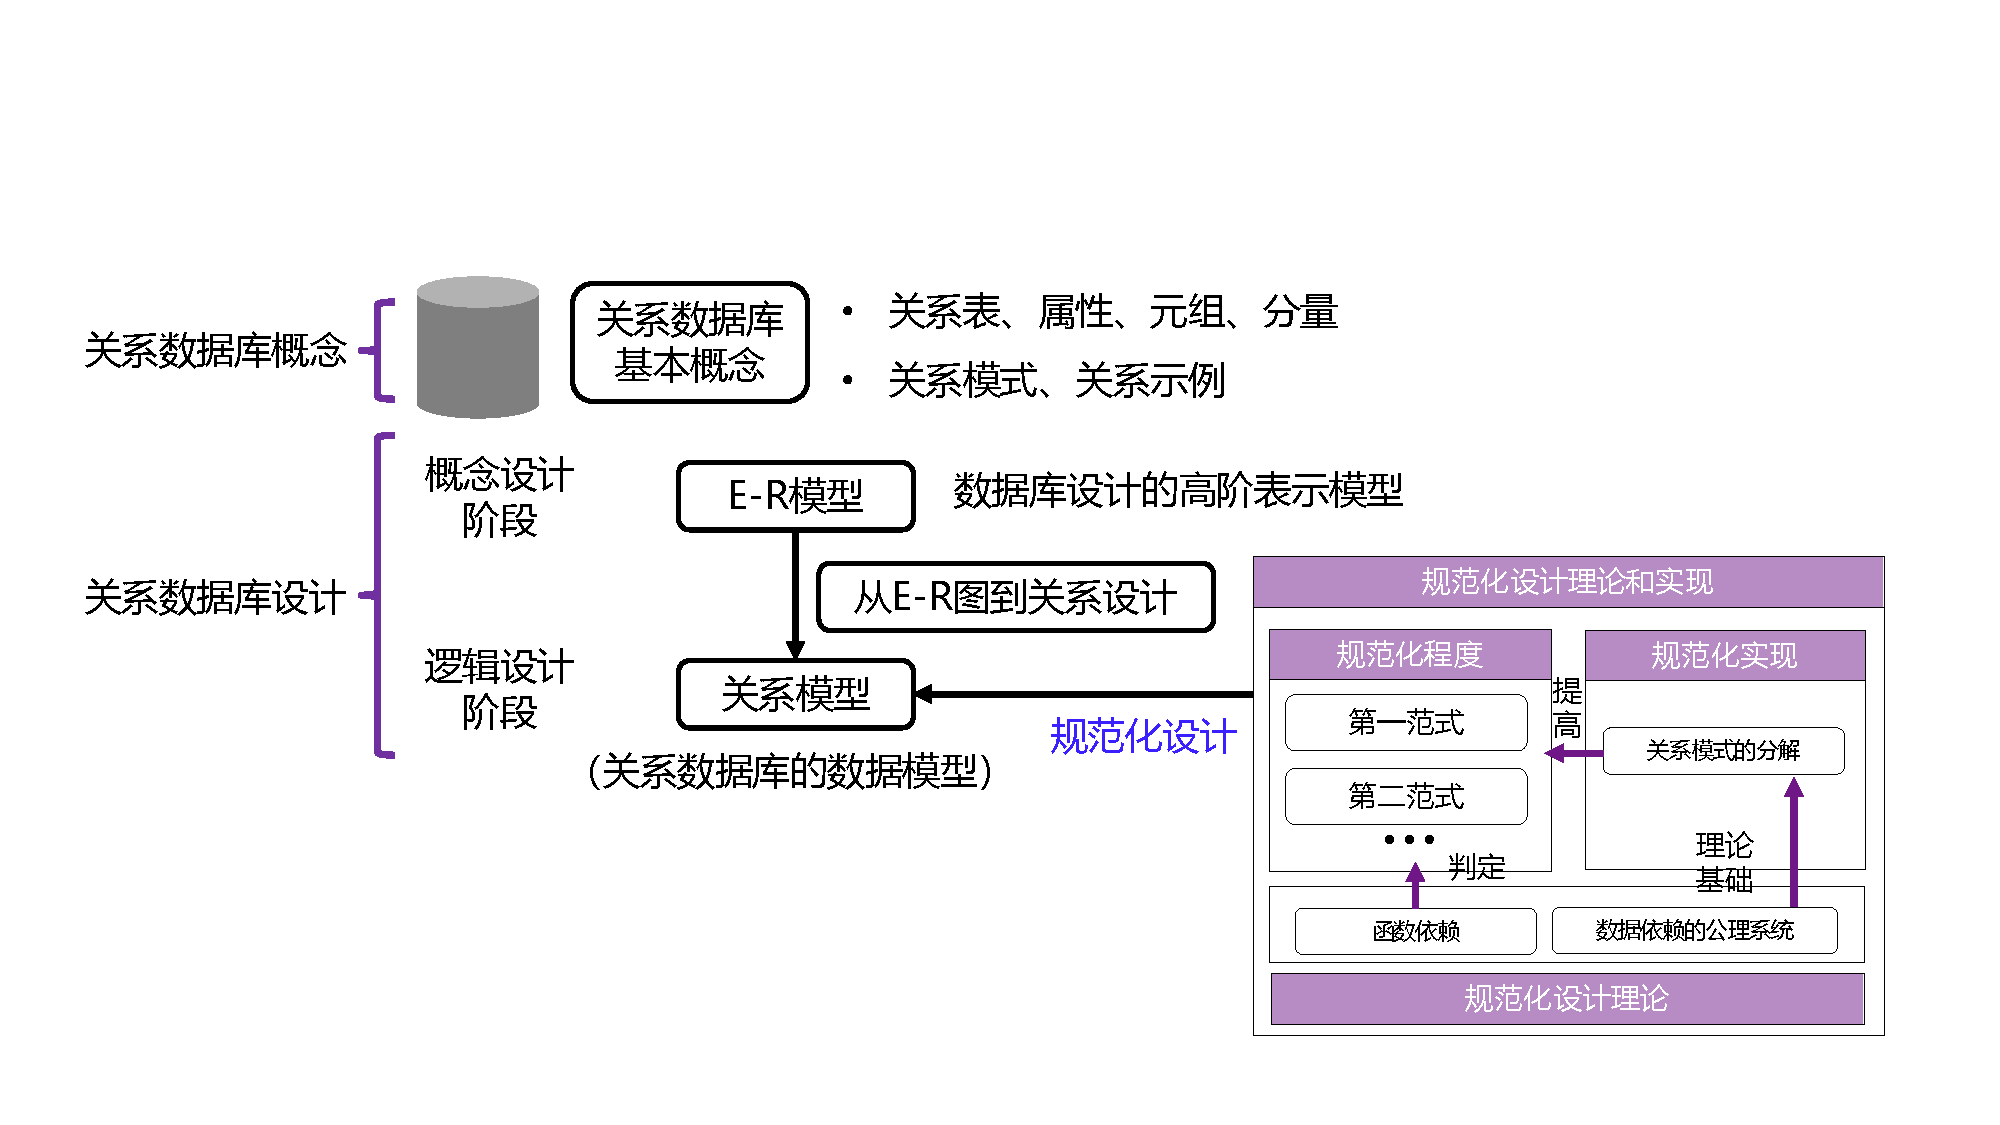
\includegraphics[width=12.5cm]{images/sec7/7-3_concept.pdf}
        \caption{重要概念之间的关系}
        \label{concept}
    \end{figure}
\end{note}

\begin{problem}
    某工厂生产若干产品,每种产品由不同的零件组成,有的零件可用在不同的产品上. 这些零件由不同的原材料制成,不同零件所用的材料可以相同. 这些零件按所属的不同产品分别放在仓库中,原材料按照类别放在若干仓库中. 请用E-R图画出此工厂产品、零件、材料、仓库的概念模型.
\end{problem}

\begin{solution}
    \hyperref[ERD]{E-R图}如下所示:
    \begin{figure}[!htpb]
        \centering
        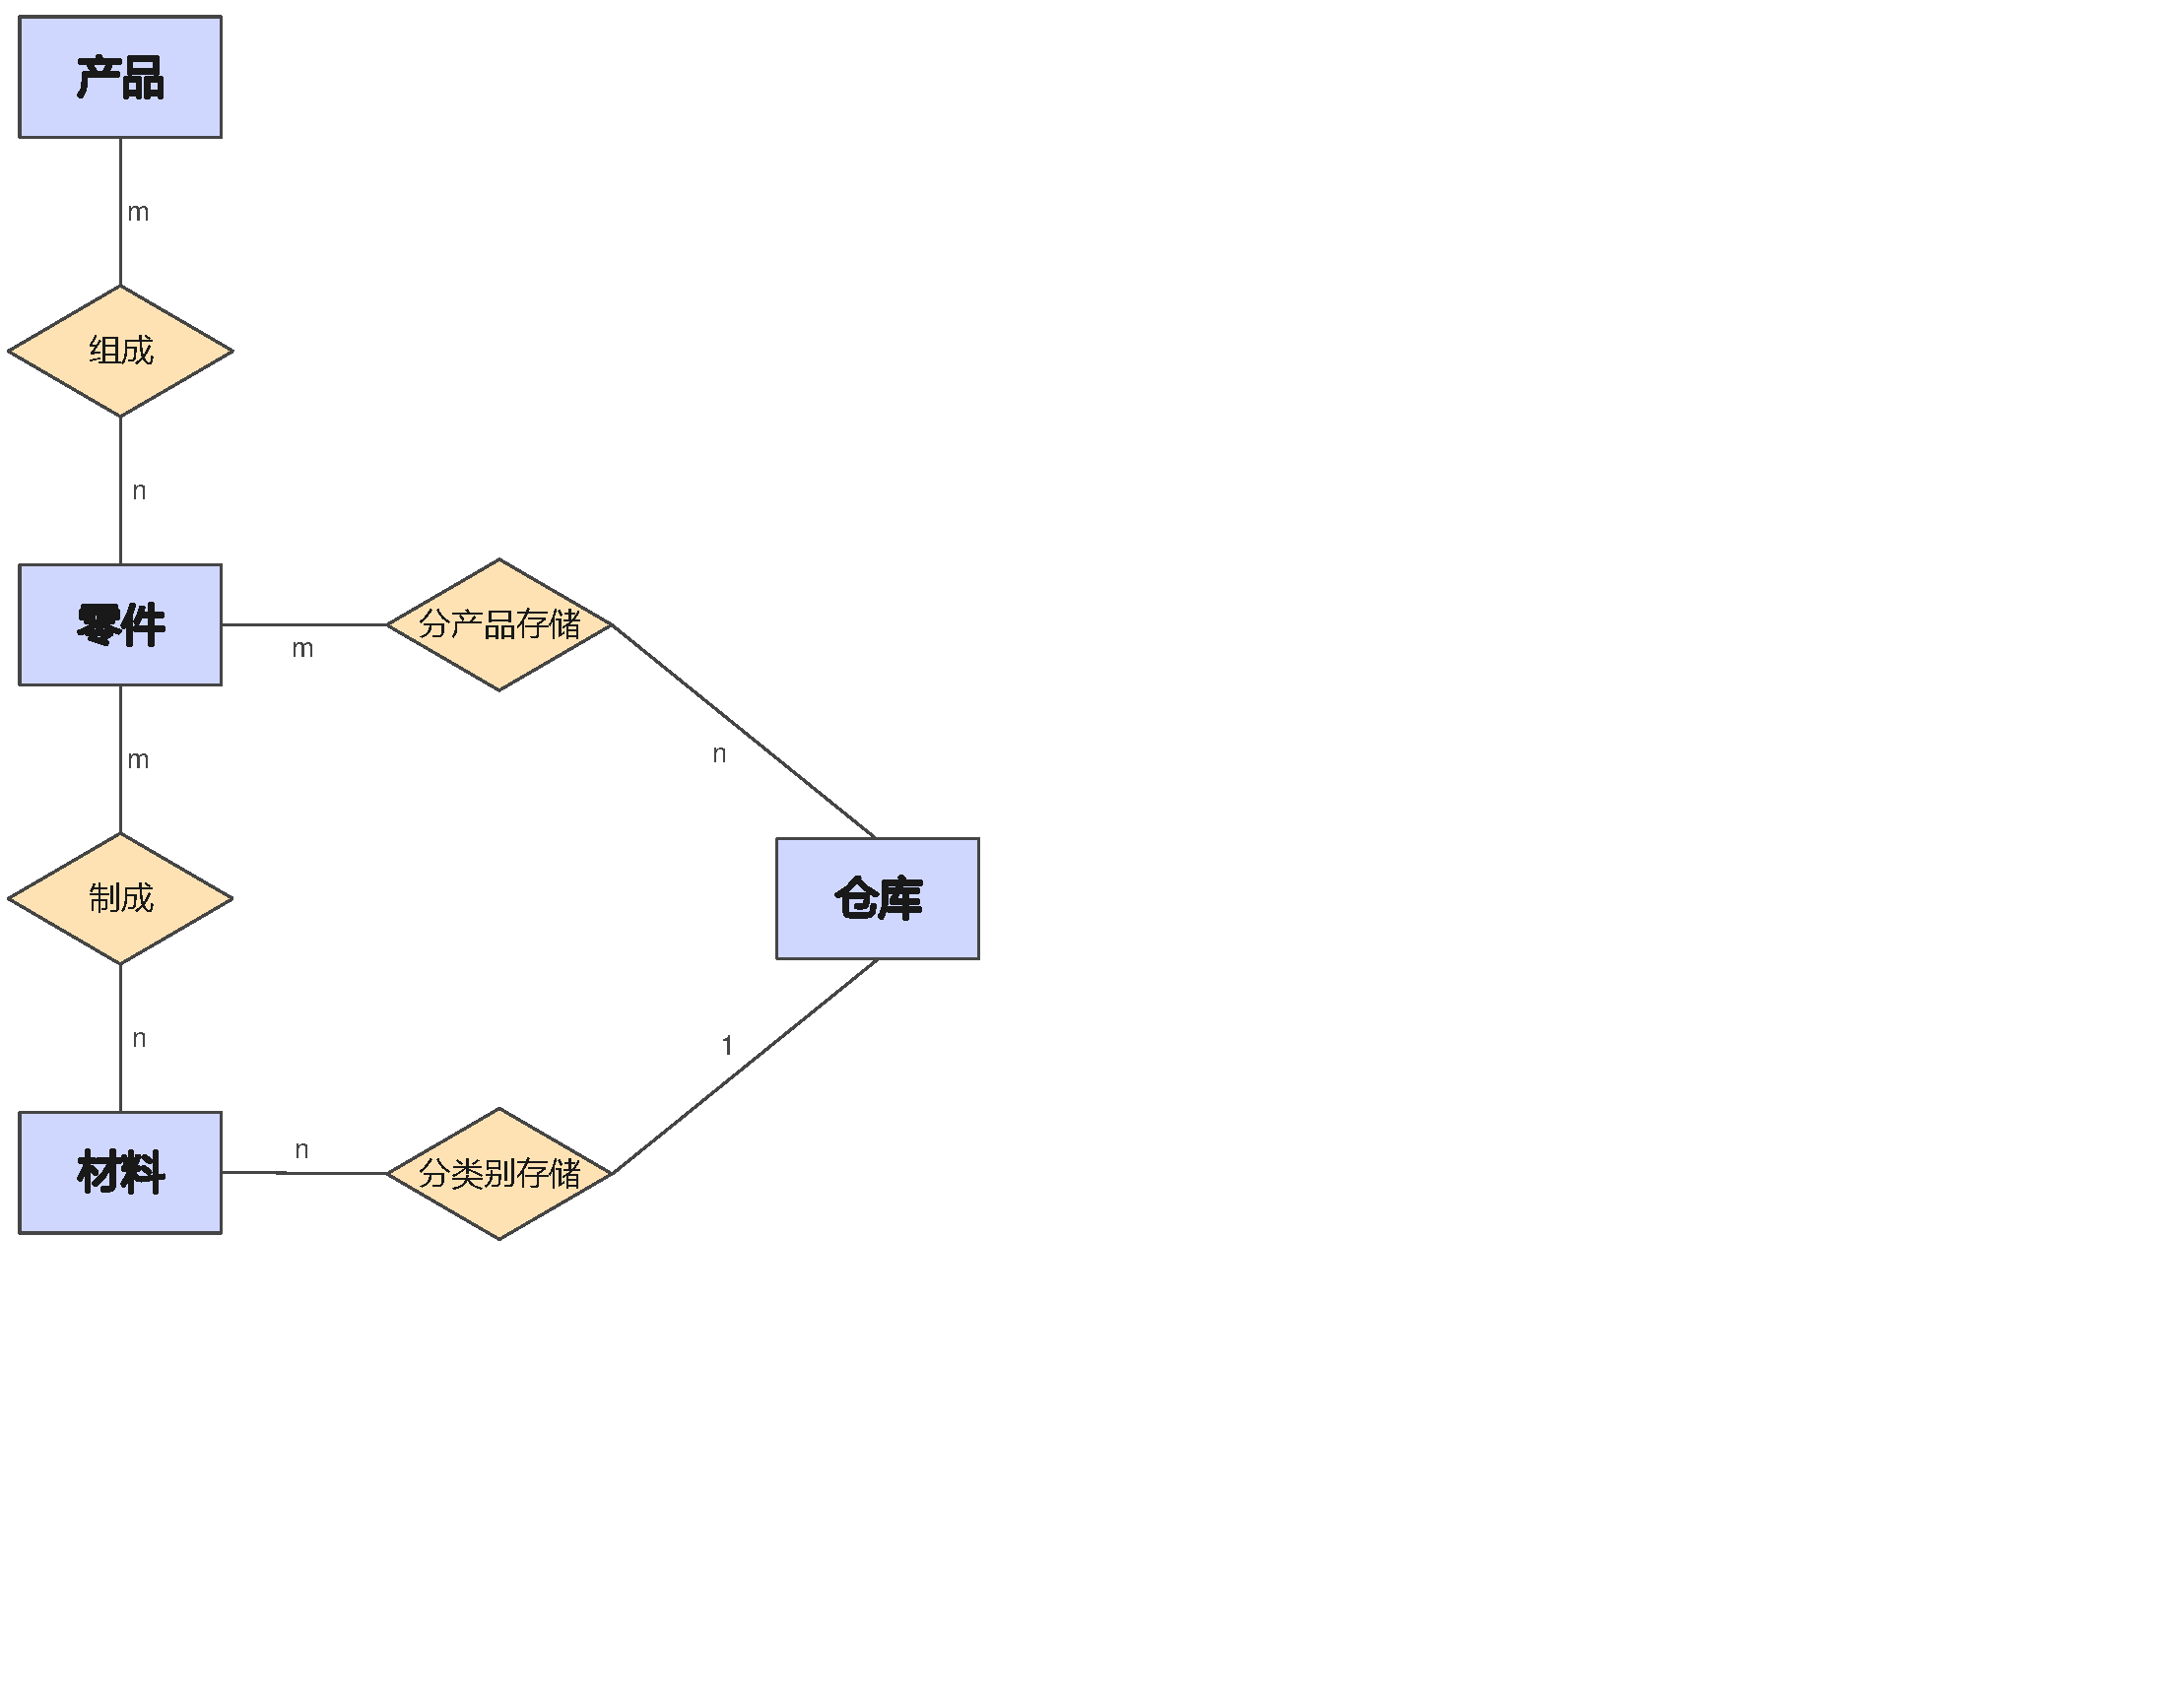
\includegraphics[width=13cm]{images/sec7/7-2_ER Diagram.pdf}
        \caption{E-R图}
        \label{ERD}
    \end{figure}
\end{solution}

\newpage

% 章节计数器加1
\stepcounter{section}

\section{第九章作业}

% 计数器置零
\setcounter{problemname}{0}

\begin{problem}
    分别描述当用下列方式更新 \texttt{Student} 表中记录时,\hyperref[fig:稠密索引]{图 9.1 }的稠密索引、\hyperref[fig:稀疏索引]{图 9.2 }的稀疏索引、\hyperref[fig:多级索引]{图 9.3 }的多级索引、\hyperref[fig:辅助索引]{图 9.4 }的辅助索引、\hyperref[fig:B+树索引]{图 9.5 }的$B^+$树索引和\hyperref[fig:哈希索引]{图 9.6 }的哈希索引分别是如何进行维护的.
    \begin{enumerate}[(1)]
        \item 插入\texttt{(20180016, 张婧宁, 女, 2002-1-2, 信息安全)}记录.
        \item 删除学号为\texttt{20180004}的记录.
        \item 删除学号为\texttt{20180005}的记录.
        \item 将学号为\texttt{20180008}的记录的专业改为\texttt{计算机科学与技术}.
    \end{enumerate}
\end{problem}

\begin{figure}[!htbp]
    \centering
    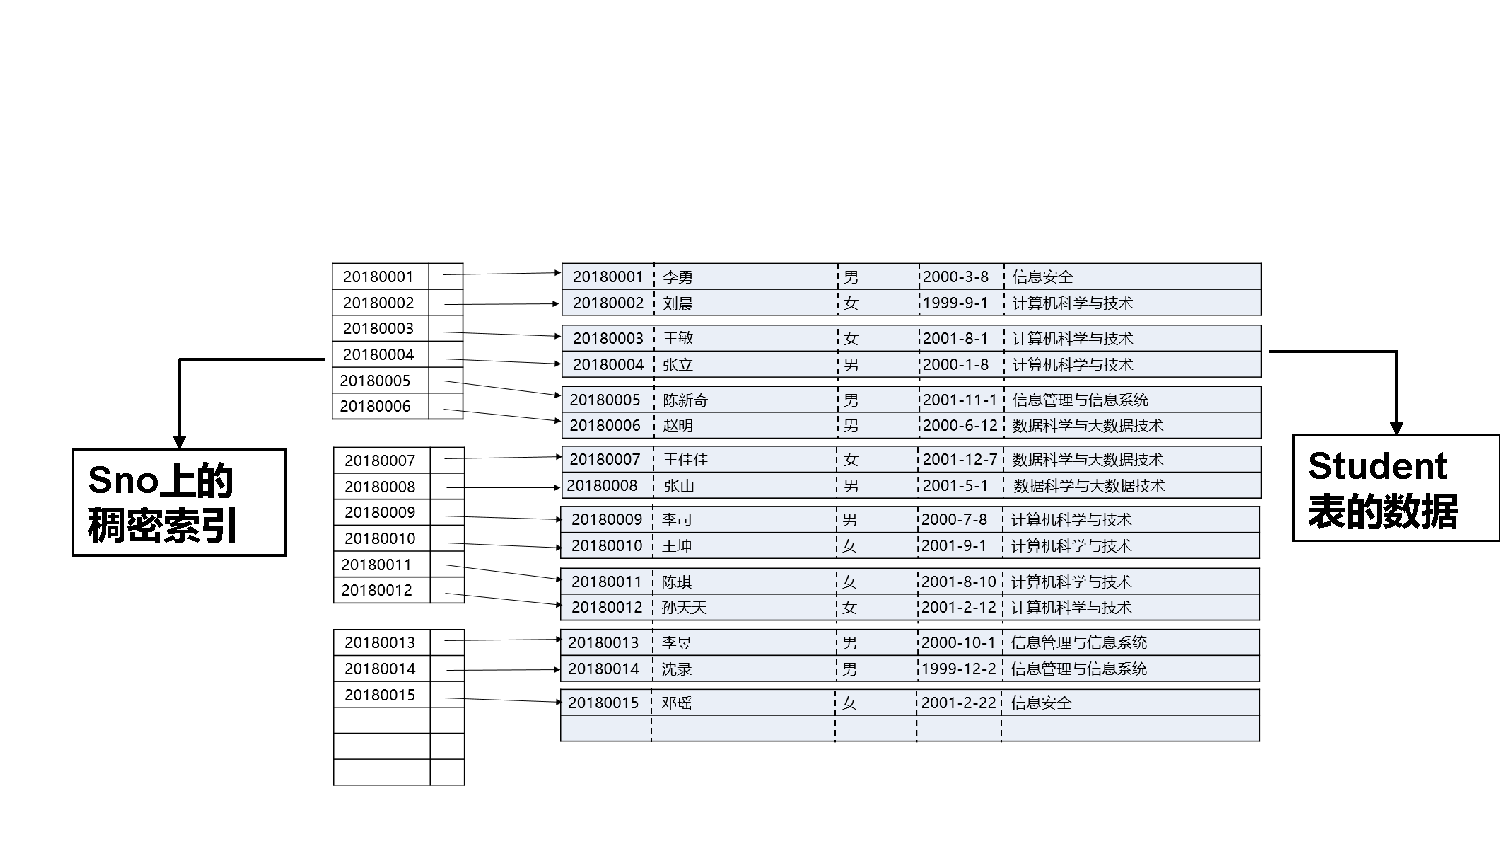
\includegraphics[width=13cm]{images/sec9/稠密索引.pdf}
    \caption{稠密索引}
    \label{fig:稠密索引}
\end{figure}

\begin{figure}[!htbp]
    \centering
    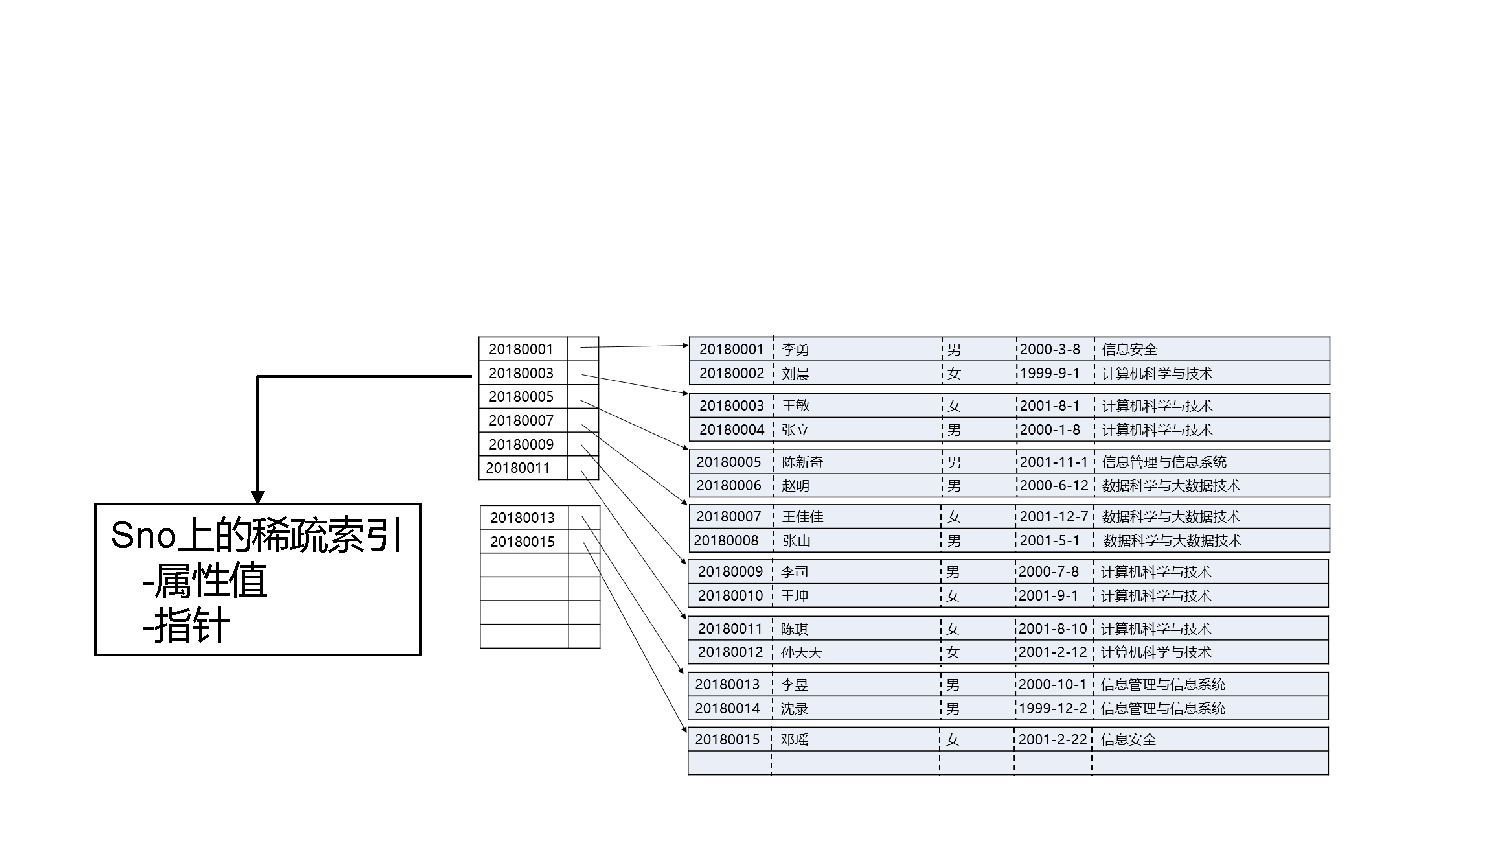
\includegraphics[width=13cm]{images/sec9/稀疏索引.pdf}
    \caption{稀疏索引}
    \label{fig:稀疏索引}
\end{figure}

\newpage

\begin{figure}[!htbp]
    \centering
    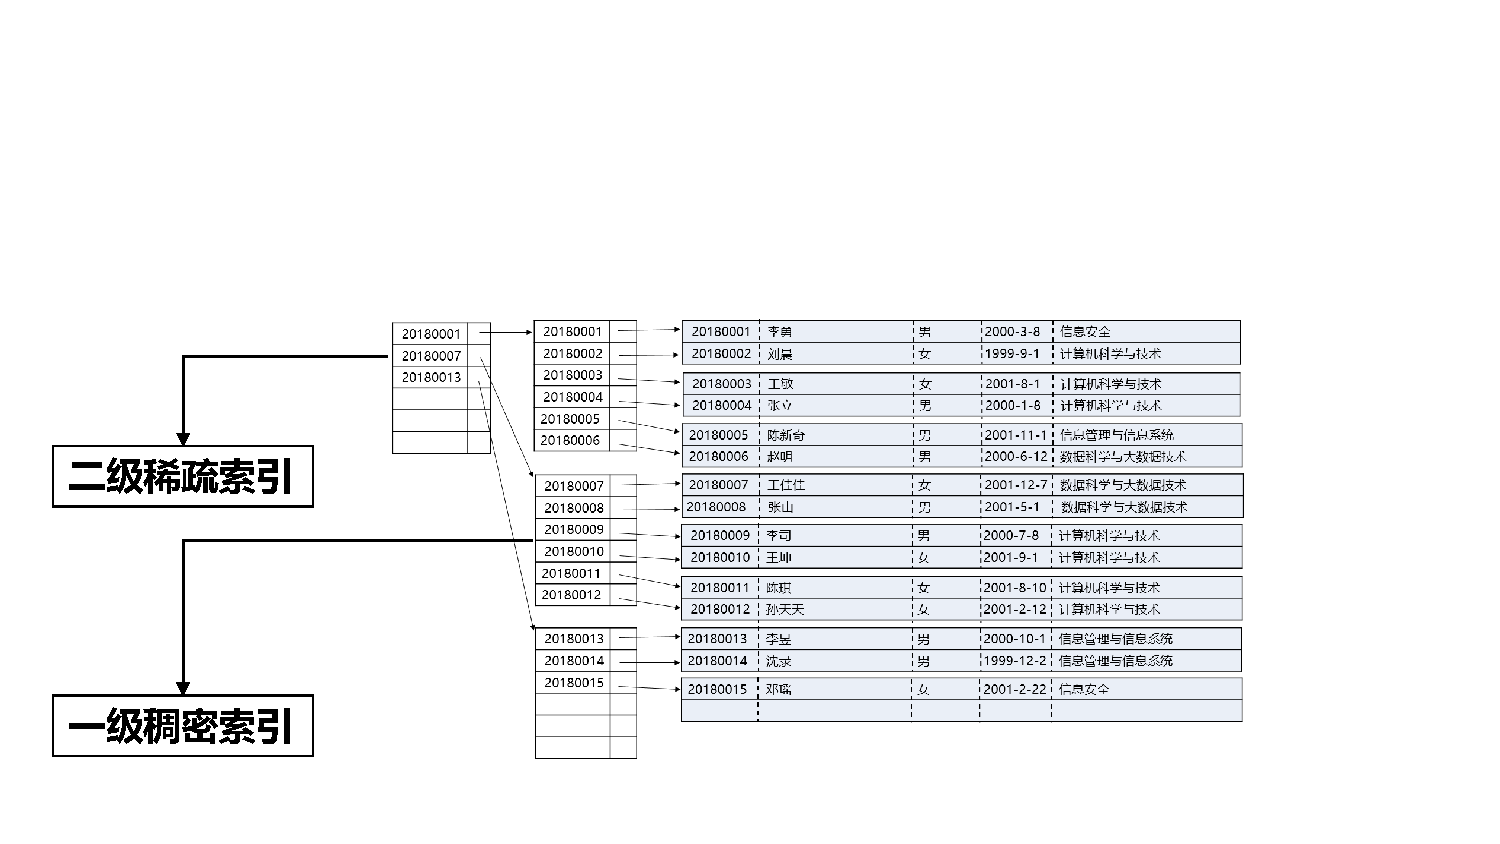
\includegraphics[width=13cm]{images/sec9/多级索引.pdf}
    \caption{多级索引}
    \label{fig:多级索引} 
\end{figure}

\begin{figure}[!htbp]
    \centering
    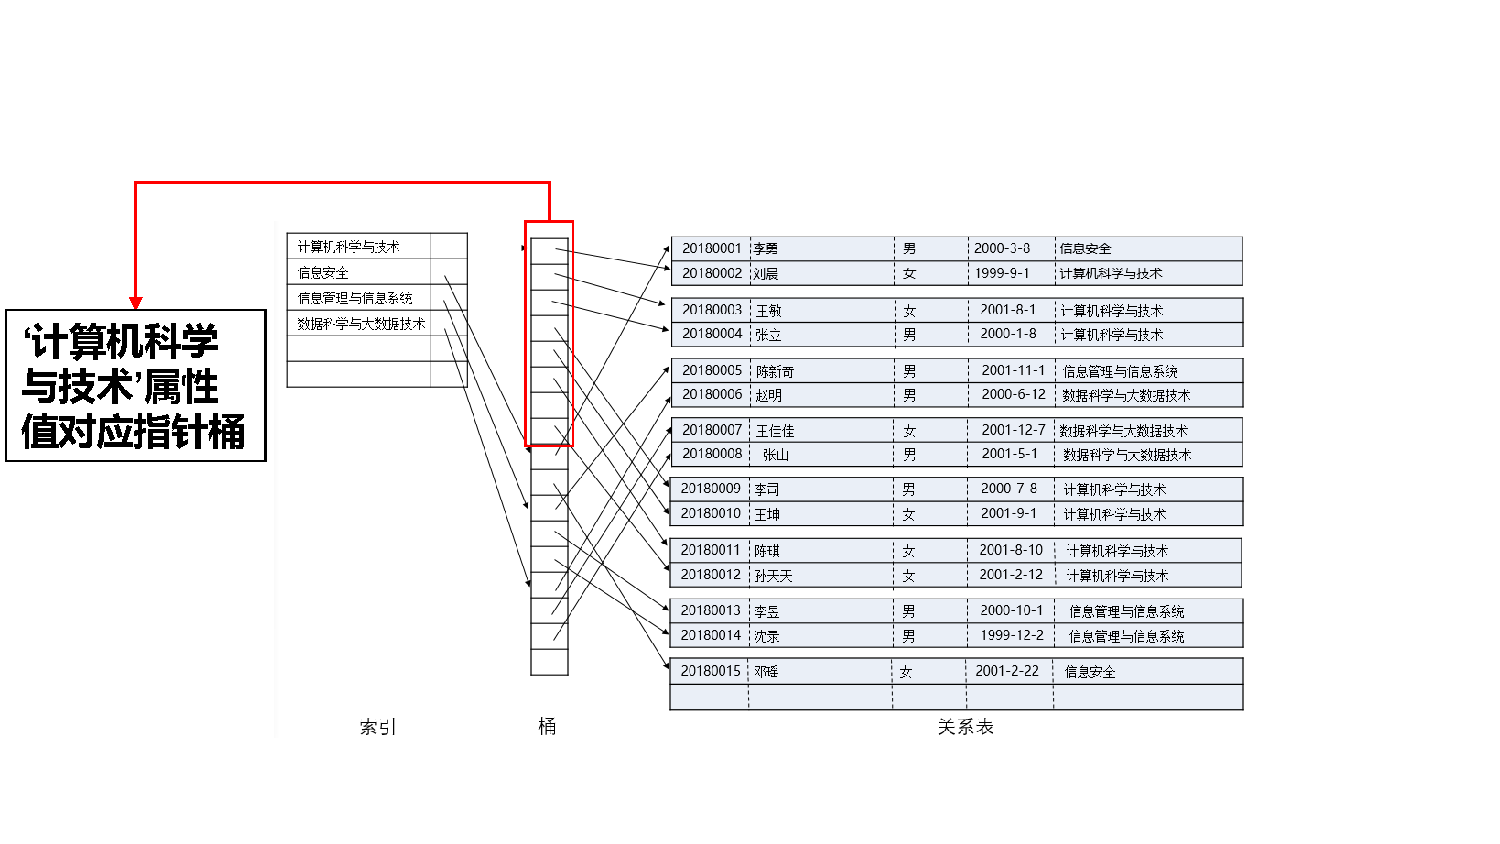
\includegraphics[width=13cm]{images/sec9/辅助索引.pdf}
    \caption{辅助索引}
    \label{fig:辅助索引}
\end{figure}

\begin{figure}[!htbp]
    \centering
    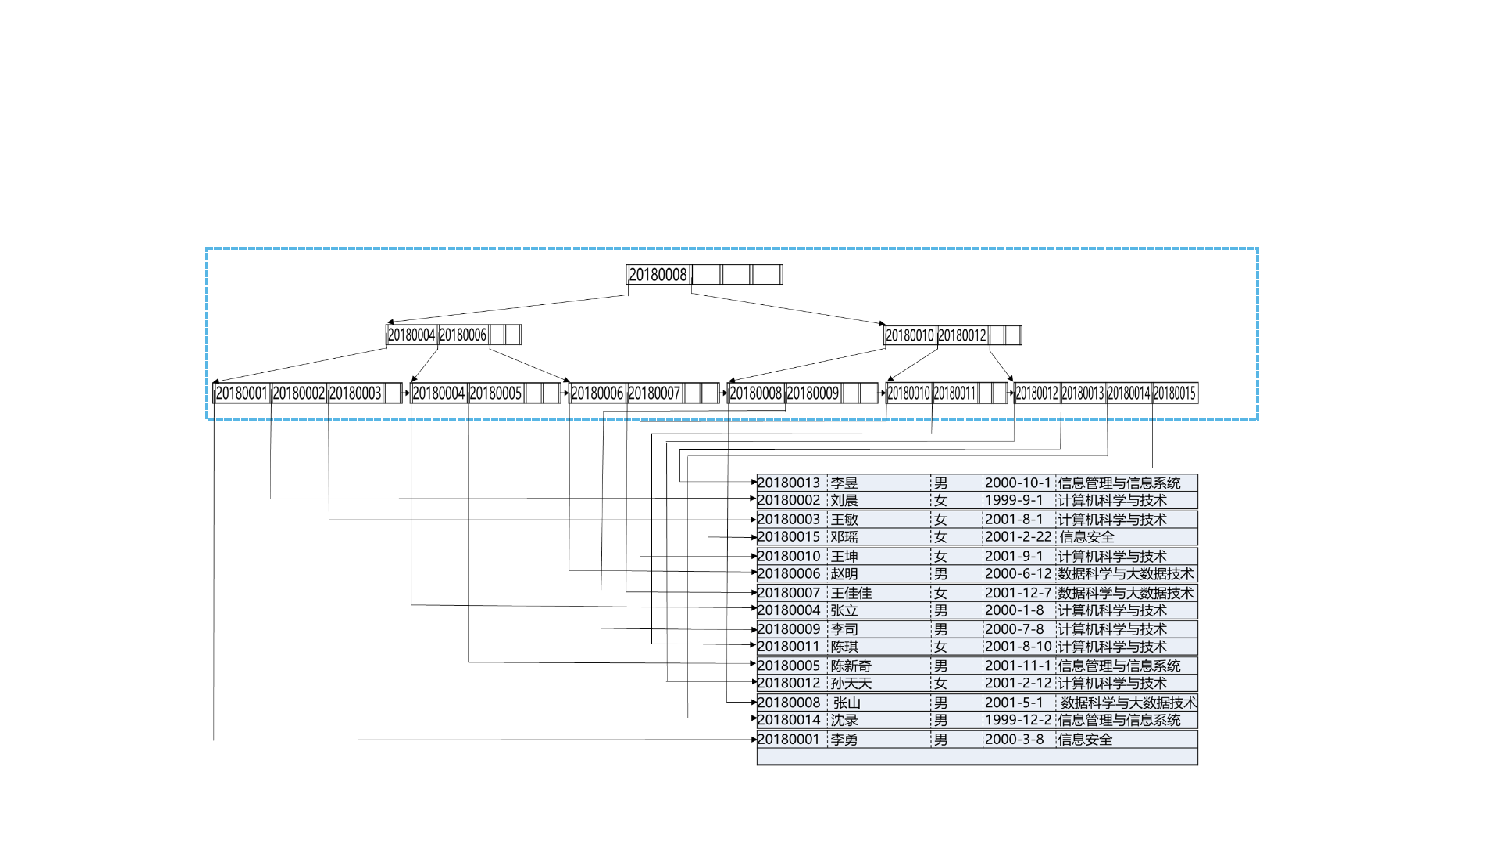
\includegraphics[width=13cm]{images/sec9/B+树索引.pdf}
    \caption{$B^+$树索引}
    \label{fig:B+树索引}
\end{figure}

\newpage

\begin{figure}[!htbp]
    \centering
    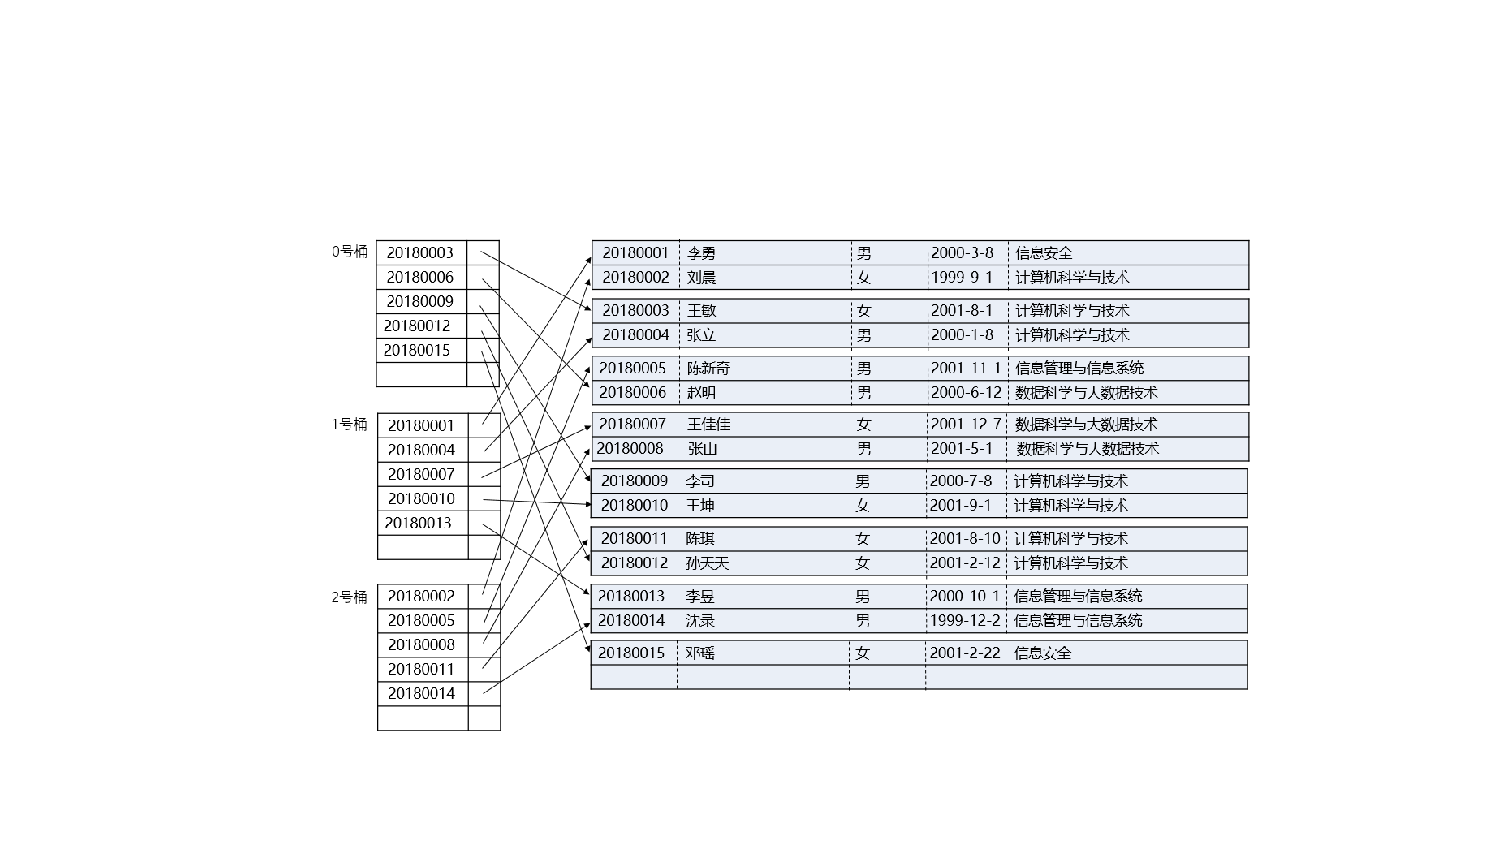
\includegraphics[width=13cm]{images/sec9/哈希索引.pdf}
    \caption{哈希索引}
    \label{fig:哈希索引}
\end{figure}

\begin{solution}
    \begin{enumerate}[(1)]
        \item 插入\texttt{(20180016, 张婧宁, 女, 2002-1-2, 信息安全)}记录.
            \begin{itemize}
                \item 稠密索引:
                
                    \qquad \texttt{Sno}索引添加新的索引\texttt{20180016}. 
                \item 稀疏索引:
                
                    \qquad \texttt{Sno}索引保持不变.
                \item 多级索引:
                
                    \qquad 二级稀疏索引保持不变,一级稠密索引添加索引\texttt{20180016}.
                \item 辅助索引:
                
                    \qquad \texttt{信息安全}对应指针桶中新增相应索引.
                \item $B^+$树索引:
                
                    \qquad 结果如\hyperref[fig:9-1-1_B+树索引]{图 9.7 }所示.
                    \begin{figure}[!htbp]
                        \centering
                        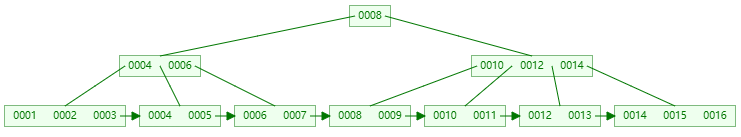
\includegraphics[width=13cm]{images/sec9/B+Tree_Case_1.png}
                        \caption{插入\texttt{20180016}后的$B^+$树索引}
                        \label{fig:9-1-1_B+树索引}
                    \end{figure}
                \item 哈希索引:
                
                    \qquad 1号桶新增索引\texttt{20180016}.
                \end{itemize}
        \item 删除学号为\texttt{20180004}的记录.
            \begin{itemize}
                \item 稠密索引:
                
                    \qquad \texttt{Sno}索引删除\texttt{20180004}.
                \item 稀疏索引:
                    
                        \qquad \texttt{Sno}索引保持不变.
                \item 多级索引:
                    
                        \qquad 二级稀疏索引保持不变,一级稠密索引删除\texttt{20180004}.
                \item 辅助索引:
                        
                        \qquad \texttt{计算机科学与技术}对应指针桶中删除相应索引.
                \item $B^+$树索引:
                            
                    \qquad 结果如\hyperref[fig:9-1-2_B+树索引]{图 9.8 }所示.
                            \begin{figure}[!htbp]
                                \centering
                                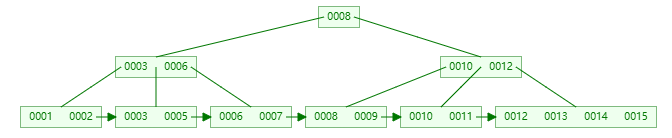
\includegraphics[width=13cm]{images/sec9/B+Tree_Case_2.png}
                                \caption{删除\texttt{20180004}后的$B^+$树索引}
                                \label{fig:9-1-2_B+树索引}
                            \end{figure}
                \item 哈希索引:
                
                    \qquad 1号桶删除索引\texttt{20180004}.
            \end{itemize}
        \item 删除学号为\texttt{20180005}的记录.
            \begin{itemize}
                \item 稠密索引:
                
                    \qquad \texttt{Sno}索引删除\texttt{20180005}.
                \item 稀疏索引:
                    
                    \qquad \texttt{Sno}索引保留\texttt{20180005},删除表中的相应数据.
                \item 多级索引:
                
                    \qquad 二级稀疏索引保持不变,一级稠密索引删除\texttt{20180005}.
                \item 辅助索引:
                
                    \qquad \texttt{信息管理与信息系统}对应指针桶中删除相应索引.
                \newpage
                \item $B^+$树索引:
                
                    \qquad 结果如\hyperref[fig:9-1-3_B+树索引]{图 9.9 }所示.
                    \begin{figure}[!htbp]
                        \centering
                        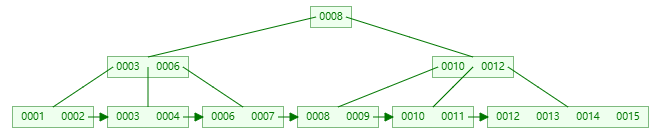
\includegraphics[width=13cm]{images/sec9/B+Tree_Case_3.png}
                        \caption{删除\texttt{20180005}后的$B^+$树索引}
                        \label{fig:9-1-3_B+树索引}
                    \end{figure}
                \item 哈希索引:
                
                    \qquad 2号桶删除索引\texttt{20180005}.
            \end{itemize}
        \item 将学号为\texttt{20180008}的记录的专业改为\texttt{计算机科学与技术}.
            \begin{itemize}
                \item 稠密索引、稀疏索引、多级索引、$B^+$树索引、哈希索引均保持不变,只需修改表中的相应数据. $B^+$树索引如\hyperref[fig:9-1-4_B+树索引]{图 9.10 }所示.
                    \begin{figure}[!htbp]
                        \centering
                        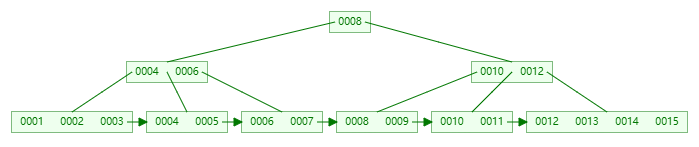
\includegraphics[width=13cm]{images/sec9/B+Tree_Case_4.png}
                        \caption{修改\texttt{20180008}后的$B^+$树索引}
                        \label{fig:9-1-4_B+树索引}
                    \end{figure}
                \item 辅助索引:
                
                    \qquad 首先从\texttt{数据科学与大数据技术}对应指针桶中删除索引\texttt{20180008},接着在\texttt{计算机科学与技术}对应指针桶中新增相应索引\texttt{20180008}.
            \end{itemize}
    \end{enumerate}
\end{solution}

\newpage
\section{第十章作业}
% 计数器置零
\setcounter{problemname}{0}

\begin{problem}
    假设关系$R(A, B)$和$S(A, B, C, D)$情况如下: $R$有20000个元组,$S$有1200个元组,一个块能装40个$R$的元组,能装30个$S$的元组,试估算下列操作需要多少次磁盘块读写.
    \begin{enumerate}[(1)]
        \item $R$上没有索引.
            \begin{Verbatim}[frame=single]
select *
from R;
            \end{Verbatim}
        \item $R$中$A$为主码,$A$有3层$B^+$树索引.
            \begin{Verbatim}[frame=single]
select *
from R
where A = 10;
            \end{Verbatim}
        
        \item 嵌套循环连接$R \bowtie S$.
        \item 排序合并连接$R \bowtie S$, 区分$R$与$S$在$B$属性上有序和无序两种情况.
    \end{enumerate}
\end{problem}

\begin{solution}
    由题可知
    \begin{equation*}
        \begin{aligned}
            & T(R) = 20000 \\
            & T(S) = 1200 \\
            & B(R) = \frac{20000}{40} = 500 \\
            & B(S) = \frac{1200}{30} = 40 \\
        \end{aligned}
    \end{equation*}
    \begin{enumerate}[(1)]
        \item 无索引下的范围选择使用线性扫描,该运算的磁盘搜索块数为$B(R)$, 因此磁盘I/O代价为$B(R)$, 即500次.
        \item 用$h_t$表示$B^+$树索引的高度,则$h_t = 3$. 接下来根据是否采用$B^+$树聚簇索引分情况讨论:
        \begin{itemize}
            \item 使用聚簇索引: 由于$B^+$树索引的结构,从磁盘中读取索引的次数为$h_t = 3$, 此外还需要执行一次磁盘读取以从磁盘中读取目标元组所在的磁盘块. 每次磁盘读取需要一次完整I/O操作,则代价可以表示为
                \begin{equation*}
                    h_t + 1 = 4
                \end{equation*}
            \item 使用非聚簇索引: 记符合选择条件的元组有$n$个. 辅助索引查找键顺序与数据文件记录顺序不一致,也就是符合选择条件的每条元组的存储位置可能位于物理位置不相邻的磁盘块. 与聚簇索引下的等值选择的区别是每条符合选择条件的元组都需要一次磁盘I/O. 所以该情况下的选择运算总代价是
                \begin{equation*}
                    h_t + n = 3 + n
                \end{equation*}
                \end{itemize}
        \item 由于关系$R$是分块读入内存,因此对于外层关系$R$的磁盘I/O次数为$B(R)$. 最外层循环是对关系$R$中的每个记录迭代,则外层循环的迭代次数为$T(R)$. 对于每次外层循环的迭代,需要按块将关系$S$读入内存,读入的内存块数为$B(S)$. 对于内层关系$S$的磁盘I/O次数为$T(R)\cdot B(S)$. 因此,嵌套循环连接的磁盘I/O总代价为
            \begin{equation*}
                B(R) + T(R) \cdot B(S) = 500 + 20000 \cdot 40 = 80500
            \end{equation*}
        \item 对于关系$R, S$是否已经排好序,分情况讨论:
            \begin{itemize}
                \item 有序: 假设两个关系$R, S$是已经排好序的关系,归并连接运算过程中只需要对两个关系顺序读取一次,因此磁盘I/O次数是
                    \begin{equation*}
                        B(R) + B(S) = 500 + 40 = 540
                    \end{equation*}
                \item 无序: 首先对关系进行排序,主要使用外部归并排序实现. 
                
                    \qquad 以关系$R$为例,假设内存中可用的块数为$M$. 排序阶段需要将关系$R$的所有元组读入内存并写回磁盘,因此排序的总磁盘I/O代价为$2B(R)$. 在归并阶段同样需要将所有元组读入内存并写回磁盘,因此每次归并阶段所需的磁盘I/O次数为$2B(R)$, 共需要$\lceil\log_{M - 1}(B(R) / M)\rceil$次归并过程. 因此外部归并排序的磁盘I/O代价为$2\left(\left\lceil\log_{M - 1}(B(R) / M)\right\rceil + 1\right) \cdot B(R)$.
                    
                    \qquad 同理,对于关系$S$也需要进行排序,排序的总磁盘I/O代价为$2B(S)$, 归并阶段的磁盘I/O代价为$2\left(\left\lceil\log_{M - 1}(B(S) / M)\right\rceil + 1\right) \cdot B(S)$.

                    \qquad 最后,进行归并连接运算. 因此,排序合并连接的磁盘I/O代价为
                        \begin{equation*}
                            \begin{aligned}
                                & 2\left(\left\lceil\log_{M - 1}(B(R) / M)\right\rceil + 1\right) \cdot B(R) \\
                                & + 2\left(\left\lceil\log_{M - 1}(B(S) / M)\right\rceil + 1\right) \cdot B(S) \\
                                & + B(R) + B(S)
                            \end{aligned}
                        \end{equation*}
            \end{itemize}
    \end{enumerate}
\end{solution}

\begin{note}
    查询处理的代价主要是指查询对各种计算资源的消耗,包括磁盘I/O占用、执行查询所用的CPU时间,如果是分布式数据库的话还需要考虑数据通信代价.

    在大型数据库系统中,磁盘I/O代价是最主要的代价,可以\textbf{使用磁盘I/O的块数作为代价度量的指标}.

    \begin{itemize}
        \item $B(R)$表示关系$R$所占用的磁盘块数.
        \item $T(R)$表示关系$R$所包含的元组条数.
        \item $M$表示可用的内存缓冲块数.
    \end{itemize}

    \begin{figure}[!htbp]
        \centering
        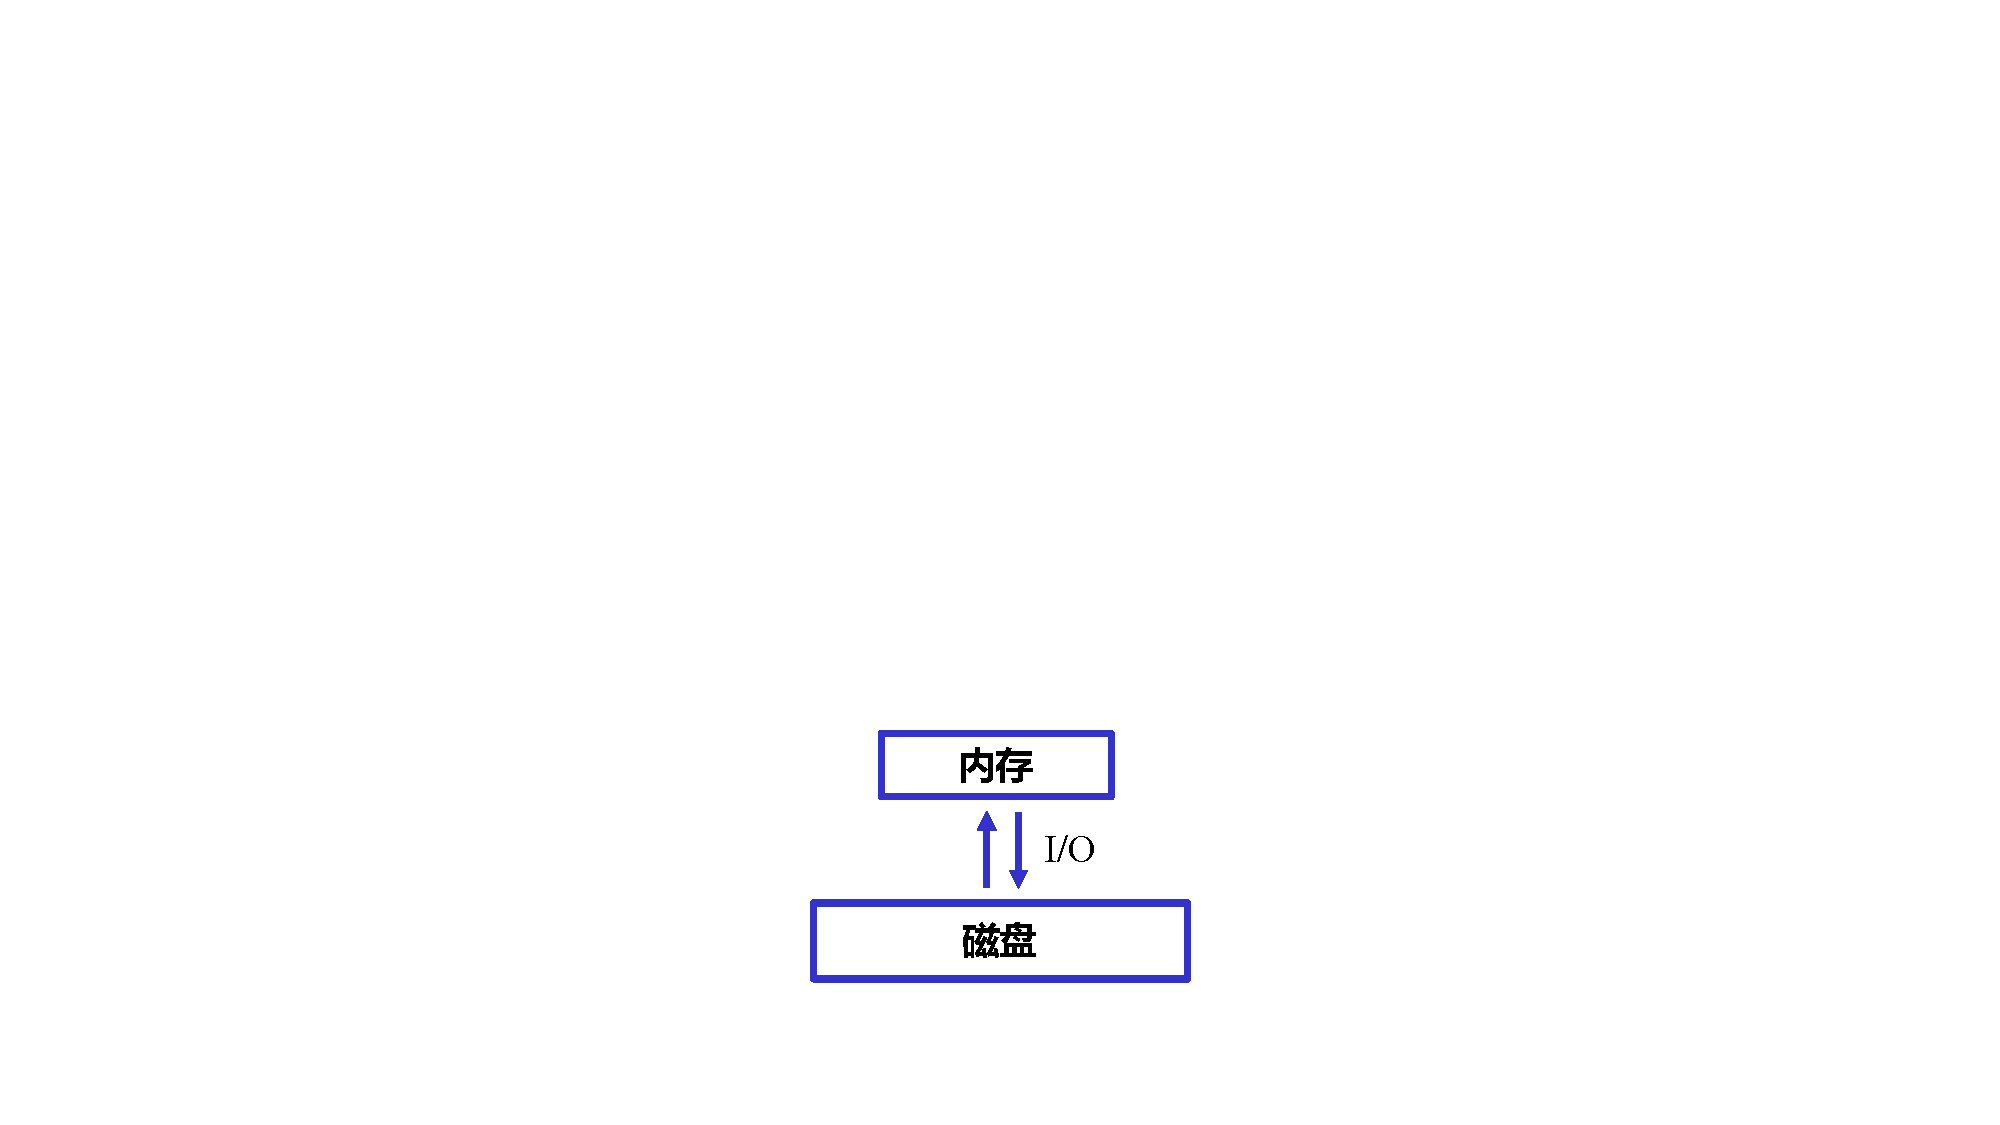
\includegraphics[width=4cm]{images/sec10/磁盘IO代价度量.pdf}
        \caption{磁盘I/O代价度量}
        \label{fig:磁盘IO代价度量}
    \end{figure}

    \begin{figure}[!htbp]
        \centering
        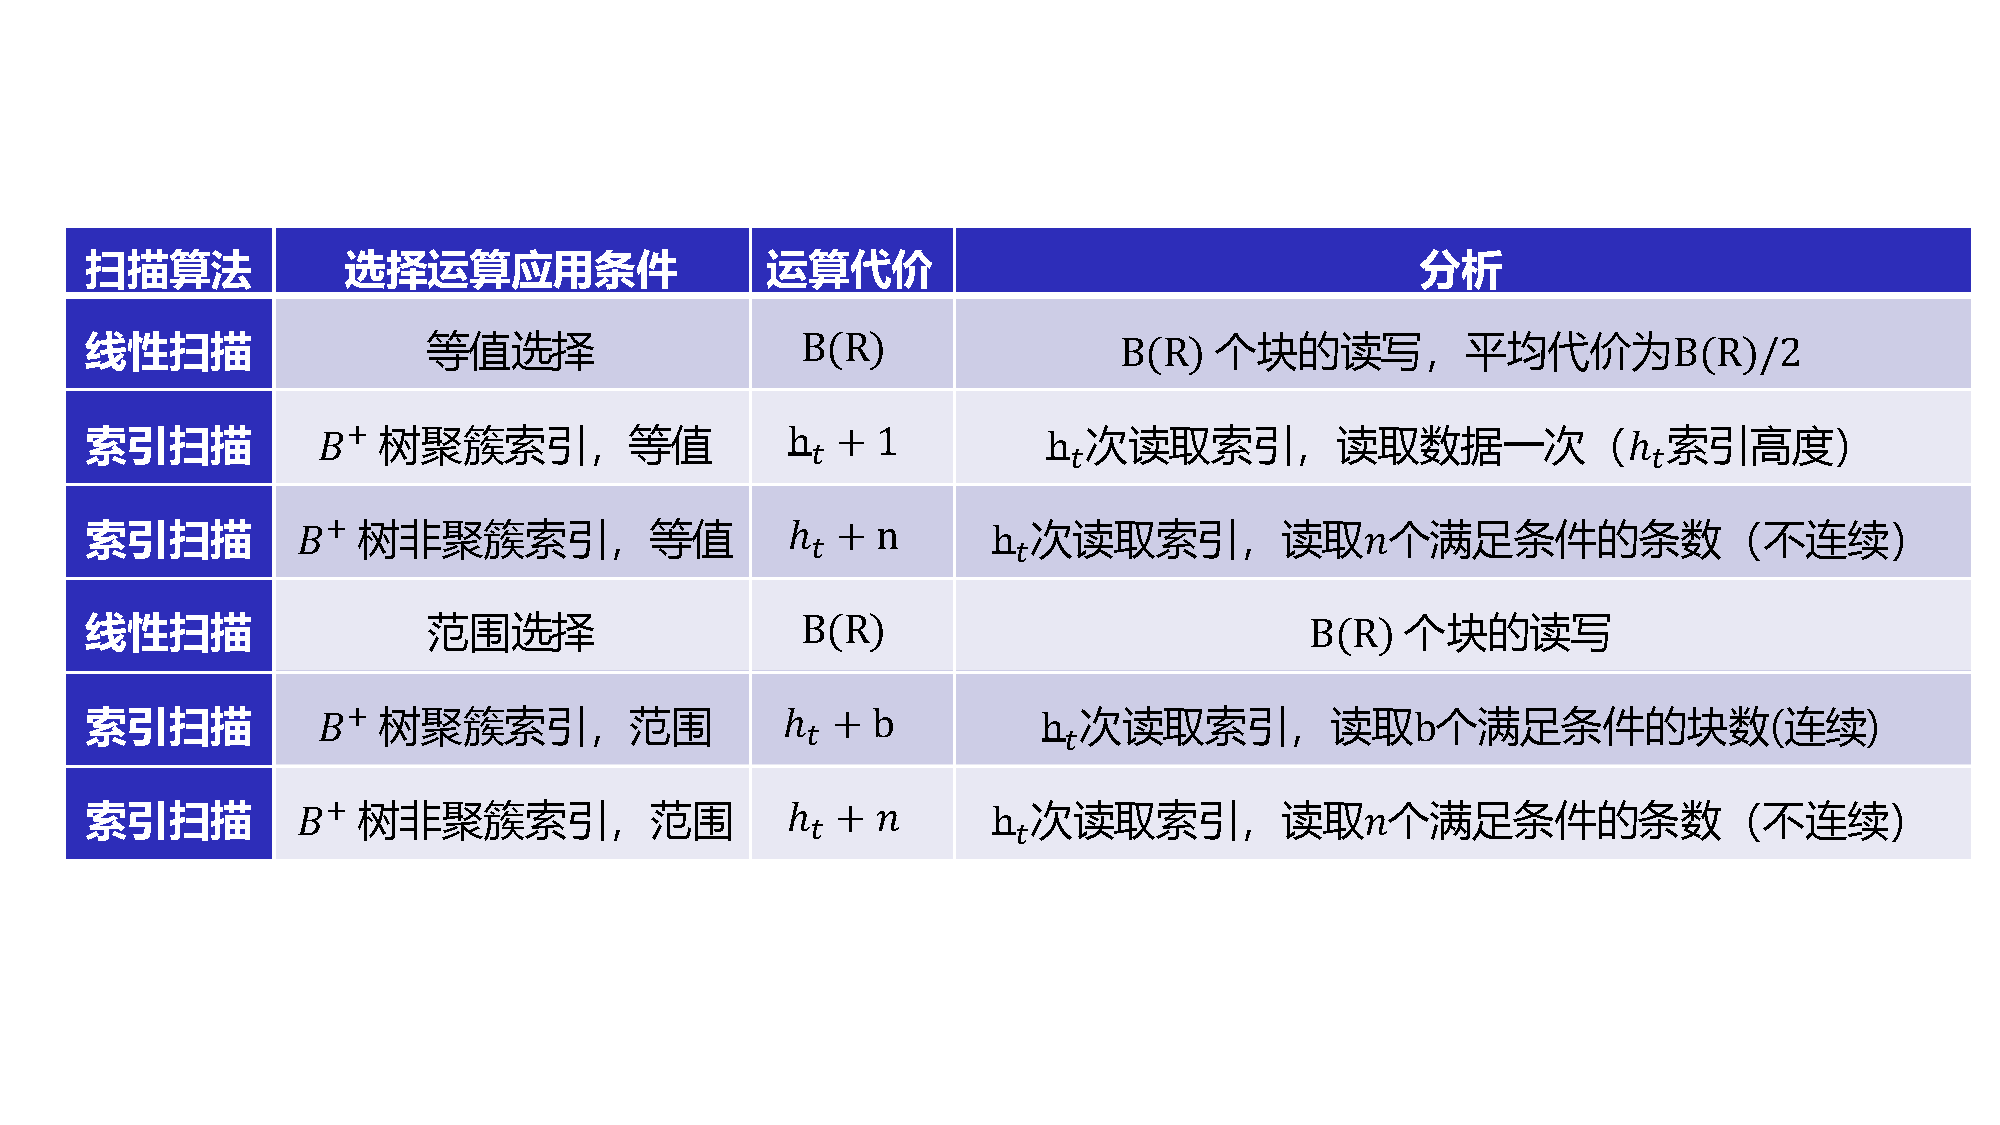
\includegraphics[width=13cm]{images/sec10/选择运算代价汇总.pdf}
        \caption{选择运算代价汇总}
        \label{fig:选择运算代价汇总}
    \end{figure}

    \begin{figure}[!htbp]
        \centering
        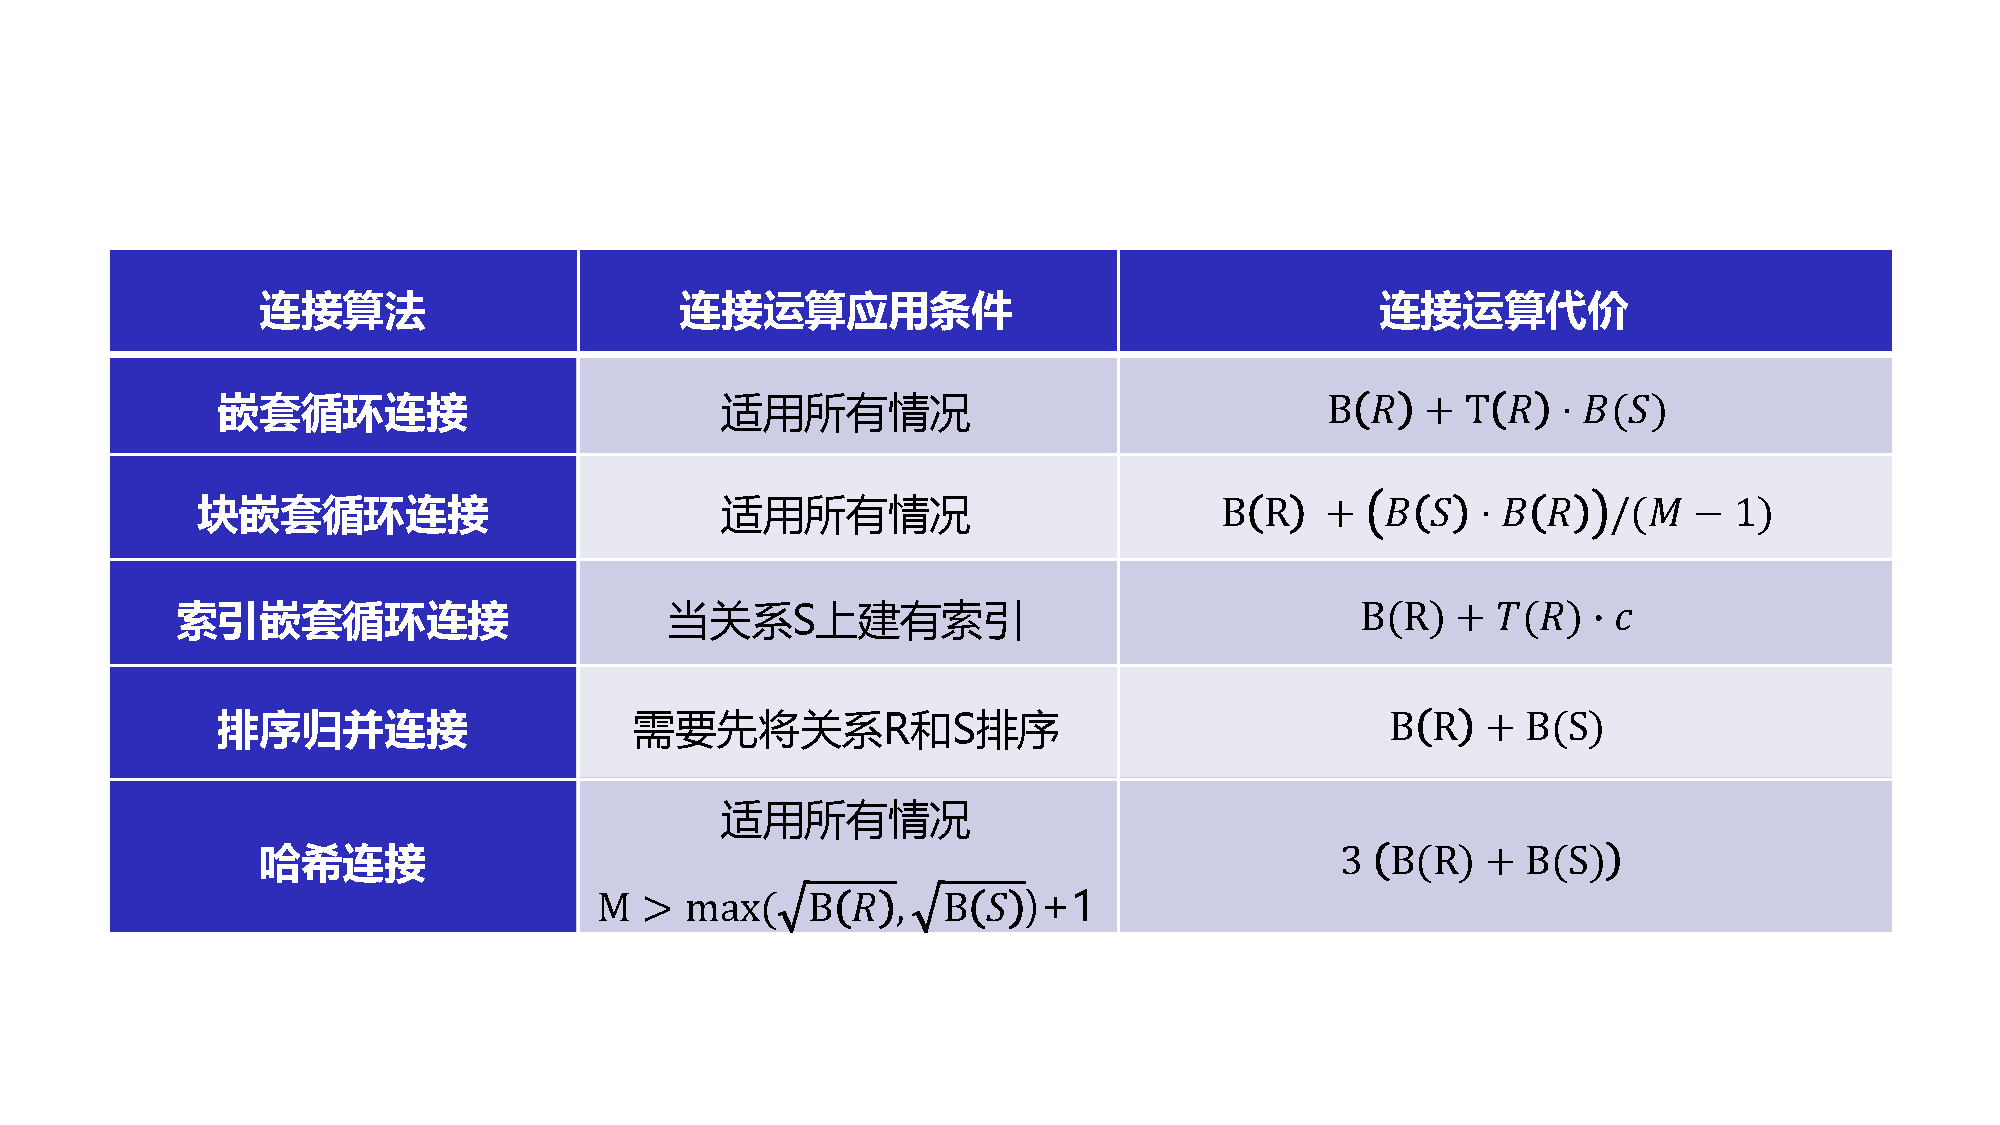
\includegraphics[width=13cm]{images/sec10/连接运算代价汇总.pdf}
        \caption{连接运算代价汇总}
        \label{fig:连接运算代价汇总}
    \end{figure}
\end{note}

\begin{problem}
    对“学生选课管理”数据库,查询信息管理与信息系统专业学生选修的所有课程名称.
    \begin{Verbatim}[frame=single]
SELECT Cname
FROM Student, Course, SC
WHERE Student.Sno = SC.Sno
    AND SC.Cno = Course.Cno
    AND Student.Smajor = '信息管理与信息系统';
    \end{Verbatim}
    试画出用关系代数表示的语法树,并用关系代数表达式优化算法对原始的语法树进行优化处理,画出优化后的标准语法树.
\end{problem}

\begin{solution}
    首先构建语法分析树,如\hyperref[fig:语法分析树]{图 10.4 }所示.
    \begin{figure}[!htpb]
        \centering
        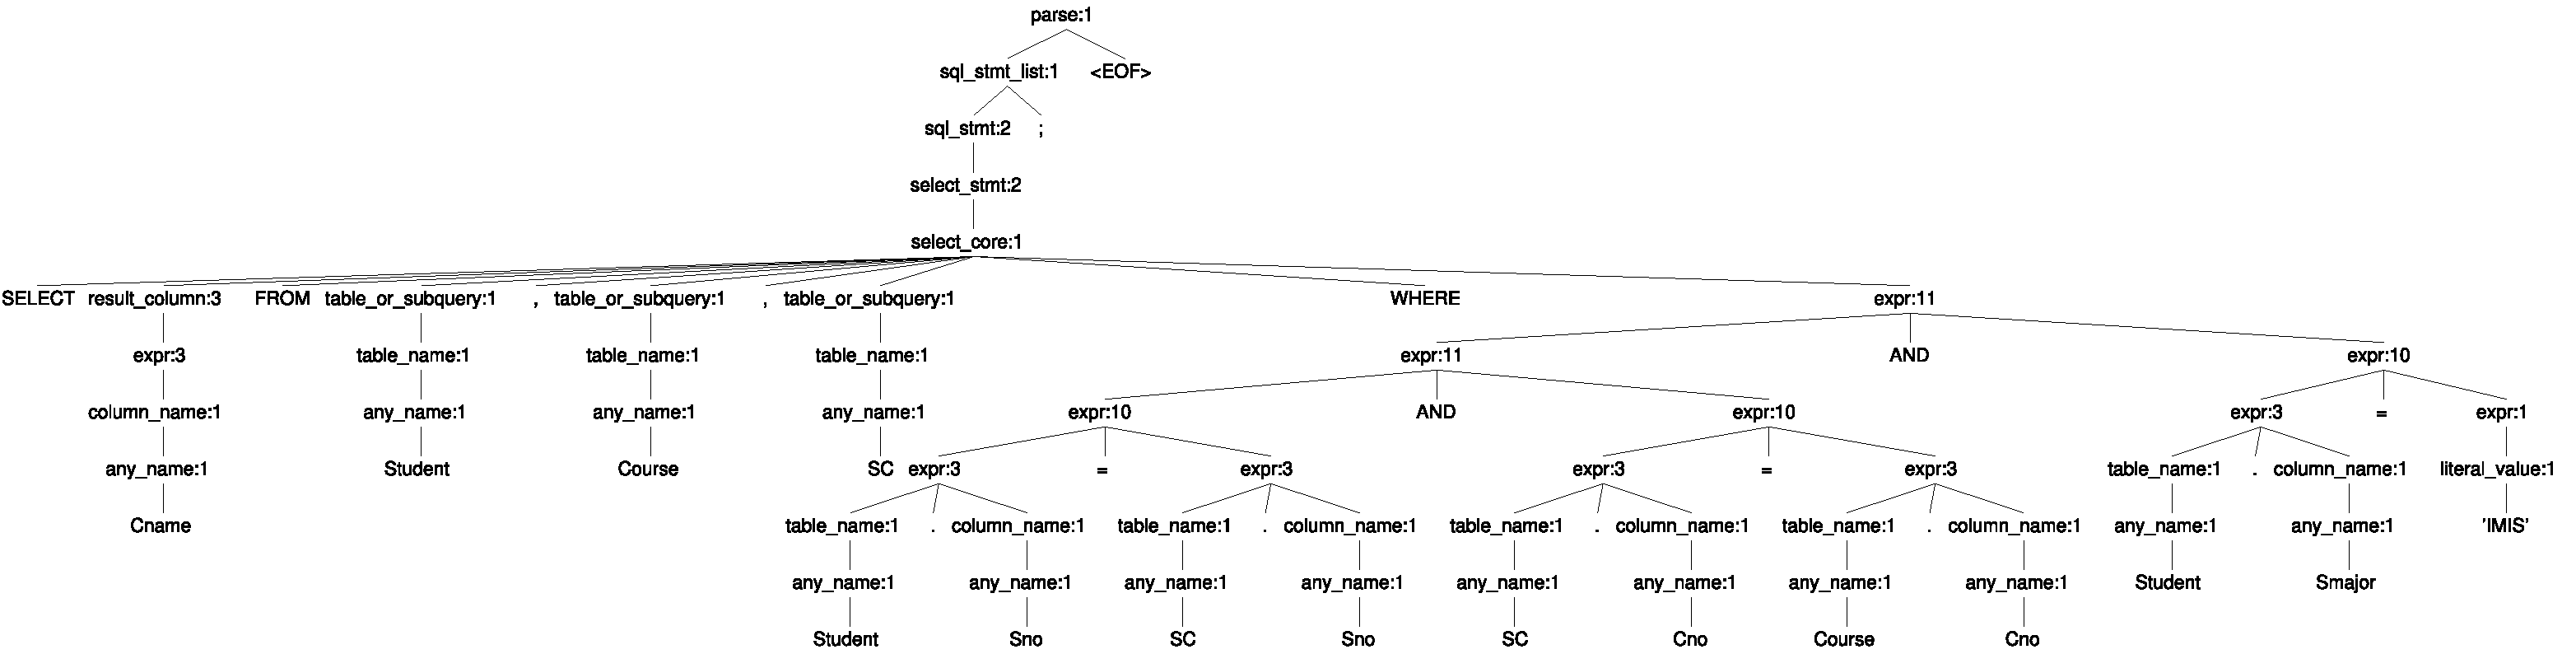
\includegraphics[width=\textwidth]{images/sec10/parser-tree.pdf}
        \caption{语法分析树}
        \label{fig:语法分析树}
    \end{figure}

    由语法分析树进行语义分析,进行语义正确性检查,并转化为查询树,如\hyperref[fig:原始查询树]{图 10.5 }所示.
    \begin{figure}[!htpb]
        \centering
        \includegraphics[width=12.5cm]{images/sec10/query-tree.jpg}
        \caption{原始查询树}
        \label{fig:原始查询树}
    \end{figure}

    使用重写规则
    \begin{equation*}
        \begin{aligned}
            & \sigma_{p_1 \land p_2}(R) = \sigma_{p_1}\left(\sigma_{p_2}\left(R\right)\right) \\
            & \sigma_p\left(R_1 \times R_2\right) = R_1 \bowtie_p R_2 \\ 
        \end{aligned}
    \end{equation*}
    尽可能多地做选择下推与笛卡尔积转连接,最终得到优化后的查询树,如\hyperref[fig:优化查询树]{图 10.6 }所示.
    \begin{figure}[!htpb]
        \centering
        \includegraphics[width=13cm]{images/sec10/optimized-query-tree.jpg}
        \caption{优化查询树}
        \label{fig:优化查询树}
    \end{figure}

    其关系代数表达式为
    \begin{equation*}
        \Pi_{Cname}\left(\left(\left(\sigma_{Smajor = '\text{信息管理与信息系统}'}\left(Student\right)\right) \bowtie_{Student.Sno = SC.Sno} SC\right) \bowtie_{SC.Cno = Course.Cno} Course\right)
    \end{equation*}
\end{solution}

\begin{note}
    \href{https://www.antlr.org/}{ANTLR}是基于LL算法实现的语法解析器生成器,用Java语言编写,使用自上而下的递归下降LL剖析器方法.
    其功能强大,支持词法分析、语法分析等多种功能. 通过学习ANTLR4语法,可以实现自定义语法解析器,实现对SQL语句的解析.

    \href{http://lab.antlr.org/}{http://lab.antlr.org/}是一个在线的ANTLR4网站,无需在本地部署ANTLR4环境,即可在线编写ANTLR4语法,生成对应的解析器. \hyperref[fig:语法分析树]{图 10.4 }就是通过ANTLR4在线工具生成的语法分析树.

    \href{https://dbis-uibk.github.io/relax/landing}{RelaX}是一个在线工具,支持 SQL 语句与关系代数表达式的相互转化,同时支持查询树的生成. \hyperref[fig:原始查询树]{图 10.5 }和\hyperref[fig:优化查询树]{图 10.6 }就是通过RelaX在线工具生成的查询树.
\end{note}

\newpage
\section{第十一章作业}
% 计数器置零
\setcounter{problemname}{0}

\begin{problem}
考虑\hyperref[log:example]{表 11.1 }所示的日志记录:
\begin{enumerate}[(1)]
    \item 如果系统故障发生在序号14之后,说明哪些事务需要重做,哪些事务需要回滚.
    \item 如果系统故障发生在序号10之后,说明哪些事务需要重做,哪些事务需要回滚.
    \item 如果系统故障发生在序号9之后,说明哪些事务需要重做,哪些事务需要回滚.
    \item 如果系统故障发生在序号7之后,说明哪些事务需要重做,哪些事务需要回滚.
\end{enumerate}
\begin{longtable}{c|l}
    \caption{日志记录实例}\label{log:example} \\
    \hline
    \textbf{序号} & \multicolumn{1}{c}{\textbf{日志}} \\
    \hline
    1  & T$_1$: 开始 \\
    2  & T$_1$: 写$A, A = 10$ \\
    3  & T$_2$: 开始 \\
    4  & T$_2$: 写$B, B = 9$ \\
    5  & T$_1$: 写$C, C = 11$ \\
    6  & T$_1$: 提交 \\
    7  & T$_2$: 写$C, C = 13$ \\
    8  & T$_3$: 开始 \\
    9  & T$_3$: 写$A, A = 8$ \\
    10 & T$_2$: 回滚 \\
    11 & T$_3$: 写$B, B = 7$ \\
    12 & T$_4$: 开始 \\
    13 & T$_3$: 提交 \\
    14 & T$_4$: 写$C, C = 12$ \\
    \hline
\end{longtable}
\end{problem}

\begin{solution}
\begin{enumerate}[(1)]
    \item
        \begin{itemize}
            \item T$_1$、T$_3$在崩溃以前就已经提交,T$_2$在崩溃以前就已经终止,因此需要被重做.
                \begin{itemize}
                    \item 日志2、4、5、7、9、11需要被重做.
                \end{itemize}
            \item T$_4$在崩溃之前没有结束,需要回滚.
                \begin{itemize}
                    \item 日志14需要回滚.
                \end{itemize}
        \end{itemize}
    \item 
        \begin{itemize}
            \item T$_1$在崩溃以前就已经提交,T$_2$在崩溃以前就已经终止,因此需要被重做.
                \begin{itemize}
                    \item 日志2、4、5、7需要被重做.
                \end{itemize}
            \item T$_3$在崩溃之前没有结束,需要回滚.
                \begin{itemize}
                    \item 日志9需要回滚.
                \end{itemize}
        \end{itemize}
    \item 
        \begin{itemize}
            \item T$_1$在崩溃以前就已经提交,T$_2$在崩溃以前就已经终止,因此需要被重做.
                \begin{itemize}
                    \item 日志2、4、5、7需要被重做.
                \end{itemize}
            \item T$_3$在崩溃之前没有结束,需要回滚.
                \begin{itemize}
                    \item 日志9需要回滚.
                \end{itemize}
        \end{itemize}
    \item 
        \begin{itemize}
            \item T$_1$在崩溃以前就已经提交,因此需要被重做.
                \begin{itemize}
                    \item 日志2、5需要被重做.
                \end{itemize}
            \item T$_2$在崩溃之前没有结束,需要回滚.
                \begin{itemize}
                    \item 日志4、7需要回滚.
                \end{itemize}
        \end{itemize}
\end{enumerate}
\end{solution}

\begin{note}
    \begin{figure}[!htbp]
        \centering
        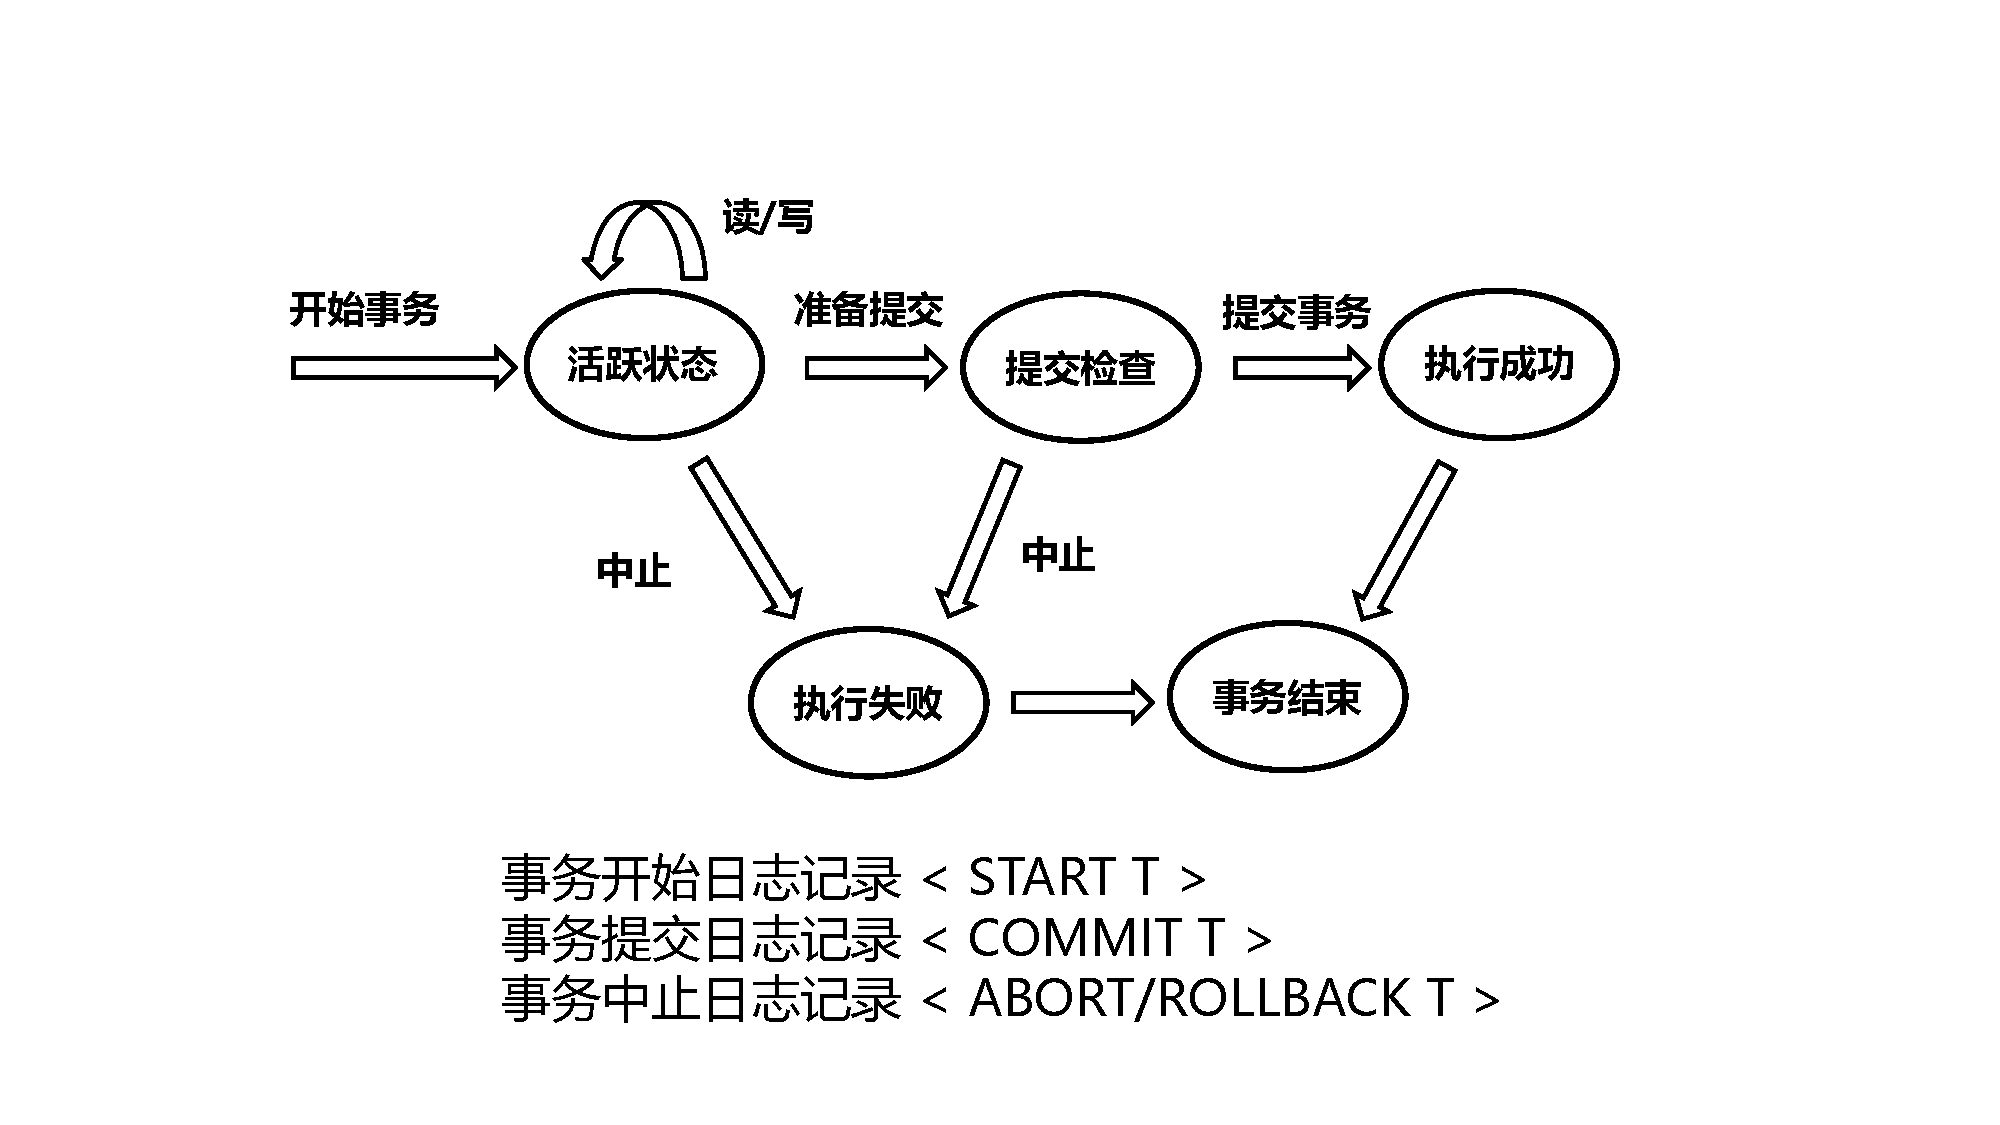
\includegraphics[width=13cm]{images/sec11/事务控制日志记录.pdf}
        \caption{事务控制日志记录}
        \label{fig:事务控制日志记录}
    \end{figure}
    \newpage
    \begin{figure}[!htbp]
        \centering
        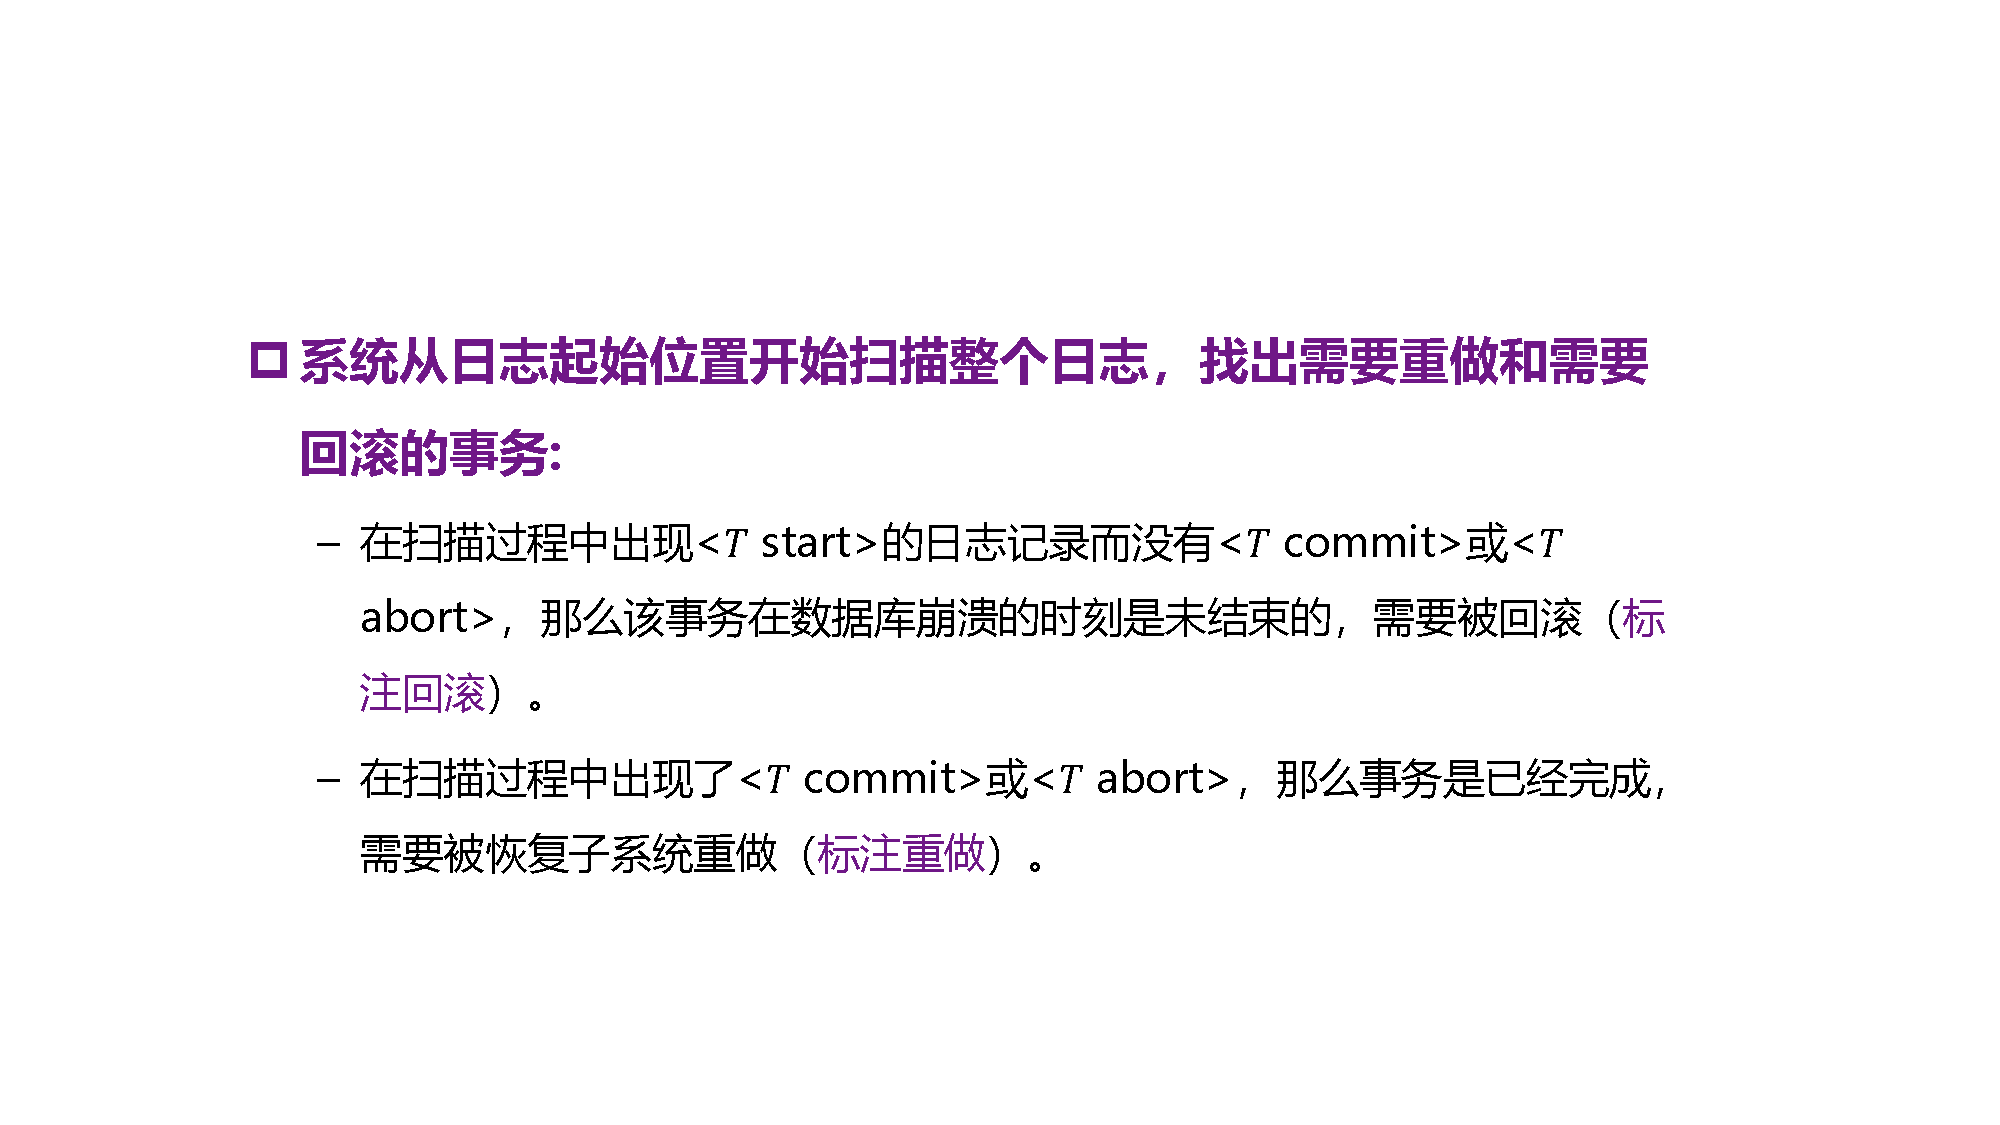
\includegraphics[width=13cm]{images/sec11/恢复分析.pdf}
        \caption{恢复分析}
        \label{fig:恢复分析}
    \end{figure}
\end{note}

\newpage
\section{第十二章作业}
% 计数器置零
\setcounter{problemname}{0}

\begin{problem}
今有三个事务的调度,如\hyperref[tab:transaction_schedule]{表 12.1 }所示,该调度是冲突可串行化的调度吗?为什么?
\begin{longtable}{c|ccc}
    \caption{事务调度}\label{tab:transaction_schedule} \\
    \textbf{时刻} & \bf $T_1$ & \bf $T_2$ & \bf $T_3$ \\
    \hline
    $t_1$ & & & $R_3(B)$ \\
    $t_2$ & $R_1(A)$ & & \\
    $t_3$ & & & $W_3(B)$ \\
    $t_4$ & & $R_2(B)$ & \\
    $t_5$ & & $R_2(A)$ & \\
    $t_6$ & & $W_2(B)$ & \\
    $t_7$ & $R_1(B)$ & & \\
    $t_8$ & $W_1(A)$ & & \\
\end{longtable}
\end{problem}

\begin{solution}
    \begin{enumerate}[$1^\circ$]
        \item 交换$t_1$与$t_3$的顺序,得到
            \begin{longtable}{c|ccc}
                \textbf{时刻} & \bf $T_1$ & \bf $T_2$ & \bf $T_3$ \\
                \hline
                $t_1$ & & & $R_3(B)$ \\
                $t_2$ & & & $W_3(B)$ \\
                $t_3$ & $R_1(A)$ & & \\
                $t_4$ & & $R_2(B)$ & \\
                $t_5$ & & $R_2(A)$ & \\
                $t_6$ & & $W_2(B)$ & \\
                $t_7$ & $R_1(B)$ & & \\
                $t_8$ & $W_1(A)$ & & \\
            \end{longtable}
        \item 交换$t_3$与$t_4$的顺序,得到
            \begin{longtable}{c|ccc}
                \textbf{时刻} & \bf $T_1$ & \bf $T_2$ & \bf $T_3$ \\
                \hline
                $t_1$ & & & $R_3(B)$ \\
                $t_2$ & & & $W_3(B)$ \\
                $t_3$ & & $R_2(B)$ & \\
                $t_4$ & $R_1(A)$ & & \\
                $t_5$ & & $R_2(A)$ & \\
                $t_6$ & & $W_2(B)$ & \\
                $t_7$ & $R_1(B)$ & & \\
                $t_8$ & $W_1(A)$ & & \\
            \end{longtable}
        \item 交换$t_4$与$t_5$的顺序,得到
            \begin{longtable}{c|ccc}
                \textbf{时刻} & \bf $T_1$ & \bf $T_2$ & \bf $T_3$ \\
                \hline
                $t_1$ & & & $R_3(B)$ \\
                $t_2$ & & & $W_3(B)$ \\
                $t_3$ & & $R_2(B)$ & \\
                $t_4$ & & $R_2(A)$ & \\
                $t_5$ & $R_1(A)$ & & \\
                $t_6$ & & $W_2(B)$ & \\
                $t_7$ & $R_1(B)$ & & \\
                $t_8$ & $W_1(A)$ & & \\
            \end{longtable}
        \item 交换$t_5$与$t_6$的顺序,得到
            \begin{longtable}{c|ccc}
                \textbf{时刻} & \bf $T_1$ & \bf $T_2$ & \bf $T_3$ \\
                \hline
                $t_1$ & & & $R_3(B)$ \\
                $t_2$ & & & $W_3(B)$ \\
                $t_3$ & & $R_2(B)$ & \\
                $t_4$ & & $R_2(A)$ & \\
                $t_5$ & & $W_2(B)$ & \\
                $t_6$ & $R_1(A)$ & & \\
                $t_7$ & $R_1(B)$ & & \\
                $t_8$ & $W_1(A)$ & & \\
            \end{longtable}
    \end{enumerate}
    此时已经串行化,因此该调度是冲突可串行化的调度.
\end{solution}
\newpage
\begin{note}
    \begin{figure}[!htbp]
        \centering
        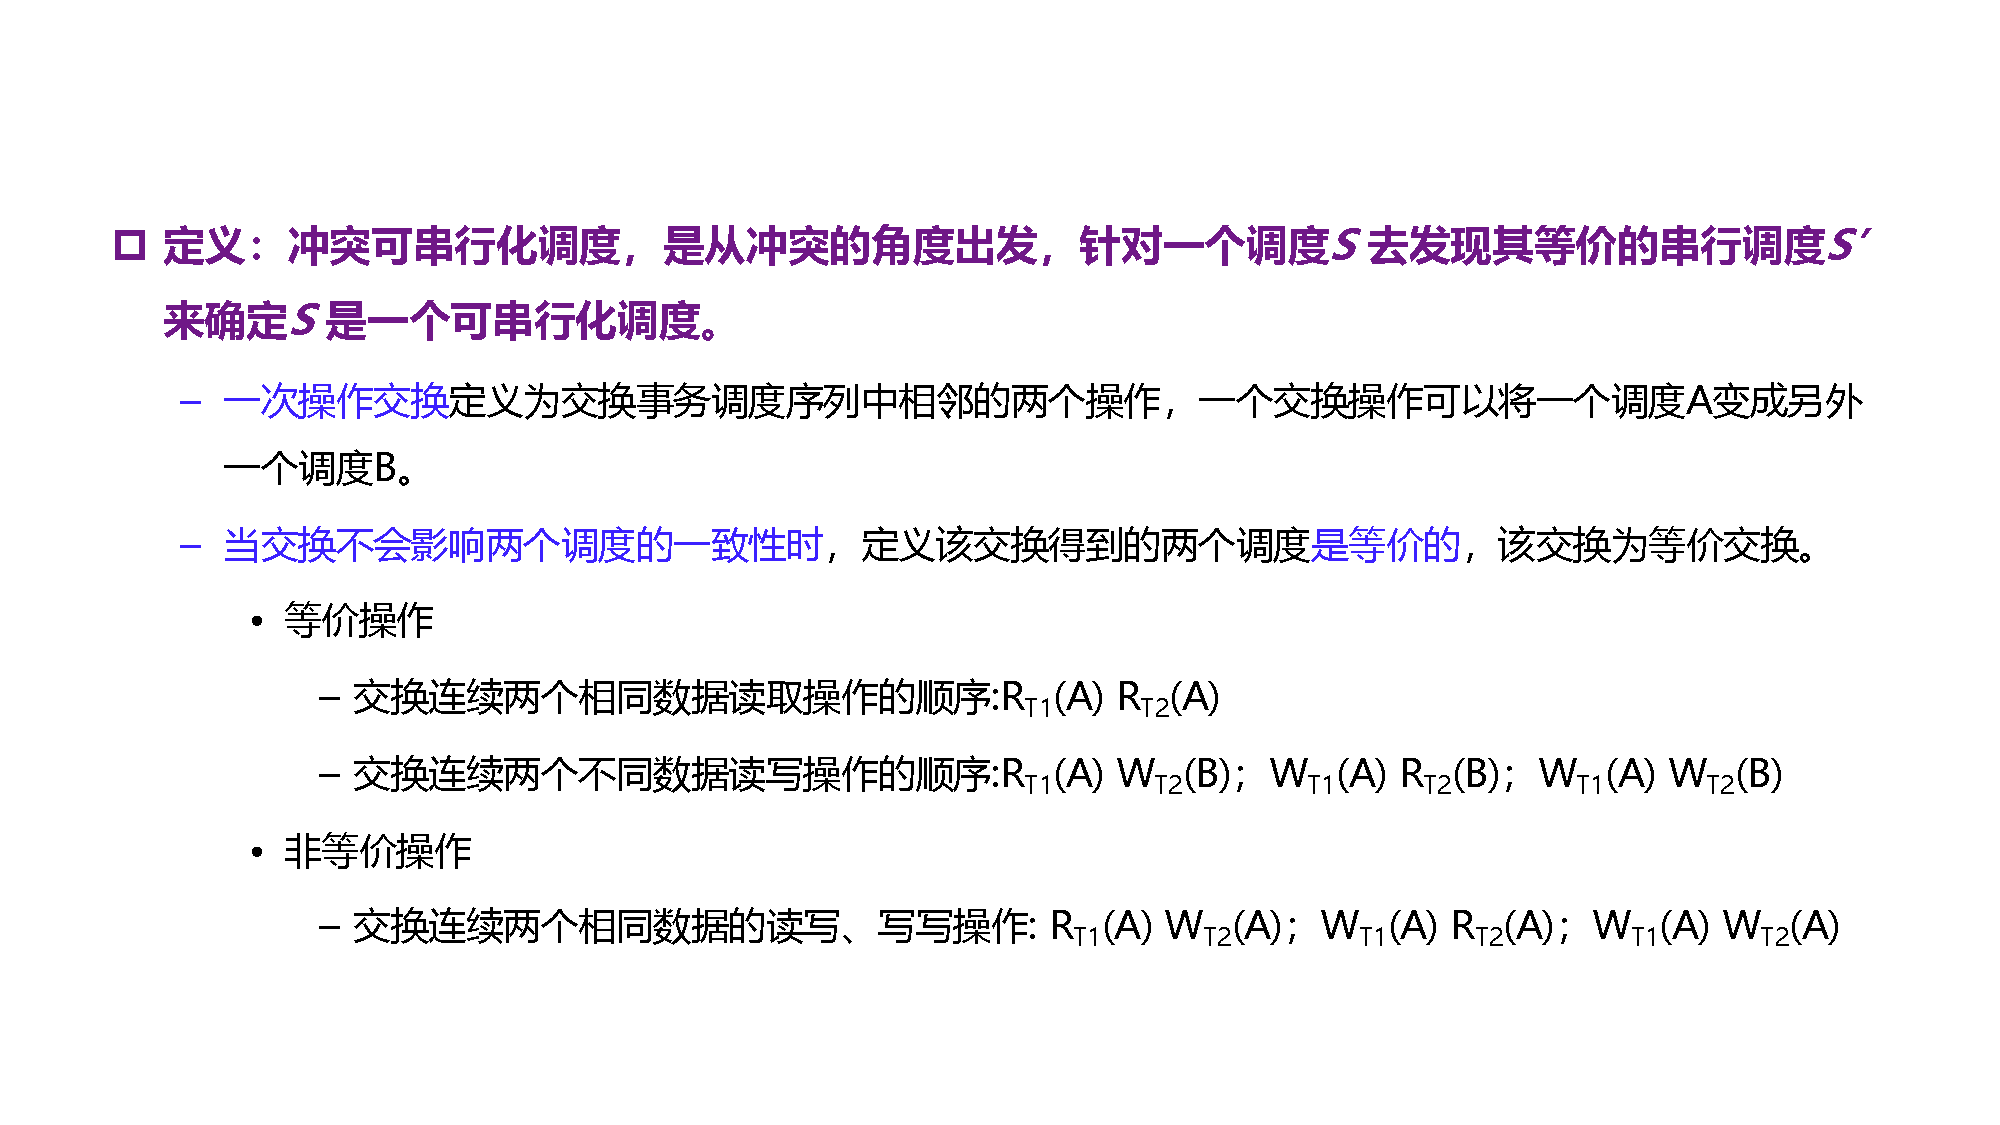
\includegraphics[width=13cm]{images/sec12/冲突可串行化调度.pdf}
        \caption{冲突可串行化调度}
        \label{fig:冲突可串行化调度}
    \end{figure}
\end{note}

% \newpage
% \section{第x章作业}
% % 计数器置零
% \setcounter{problemname}{0}

% \begin{problem}

% \end{problem}

% \begin{solution}

% \end{solution}

\end{document}